\documentclass[sigconf]{acmart}

\usepackage{booktabs} % For formal tables
\usepackage{times}
\usepackage{helvet}
\usepackage{courier}
\usepackage{graphicx}
\usepackage{multirow}
\usepackage{algorithm}
\usepackage{algorithmic}
\usepackage{mathrsfs}
\usepackage{comment}
%\newtheorem{definition}{Definition}
%\usepackage{algorithmicx}
%\usepackage{algorithm} % http://ctan.org/pkg/algorithms

% Copyright
%\setcopyright{none}
%\setcopyright{acmcopyright}
%\setcopyright{acmlicensed}
\setcopyright{rightsretained}
%\setcopyright{usgov}
%\setcopyright{usgovmixed}
%\setcopyright{cagov}
%\setcopyright{cagovmixed}


% DOI
%\acmDOI{10.475/123_4}

% ISBN
%\acmISBN{123-4567-24-567/08/06}

%Conference
%\acmConference[WOODSTOCK'97]{ACM Woodstock conference}{July 1997}{El
%  Paso, Texas USA} 
%\acmYear{2017}
\copyrightyear{2017}

%\acmPrice{15.00}


\begin{document}
\title{Temporal Motif Mining Approaches for Smart Homes}
%\titlenote{Produces the permission block, and copyright information}
%\subtitle{Extended Abstract}
%\subtitlenote{The full version of the author's guide is available as
%  \texttt{acmart.pdf} document}

\author{
  Huijuan Shao\textsuperscript{1,2}, Yaowei Li\textsuperscript{3}, Fei Li\textsuperscript{2}, Erin Griffiths \textsuperscript{4}, Kamin Whitehouse\textsuperscript{4}, Naren Ramakrishnan\textsuperscript{1,2} \\
  \textsuperscript{1}Discovery Analytics Center, Virginia Tech, Blacksburg, VA 24061 \\ %\vspace{0.1cm}
  \textsuperscript{2}Department of Computer Science, Virginia Tech, Blacksburg, VA 24061 \\ %\vspace{0.1cm}
    \textsuperscript{3} Game source, McLean, VA 22101 \\
  \textsuperscript{4}Department of Computer Science, University of Virginia, VA 22904 \\ %\vspace{0.1cm}
}




% The default list of authors is too long for headers}
\renewcommand{\shortauthors}{B. Trovato et al.}


\begin{abstract}
With the advent of modern sensor technologies, 
significant opportunities have opened up to help conserve energy in 
residential and commercial buildings. Moreover, the rapid \emph{urbanization} we are witnessing requires optimized energy distribution. 
This paper focuses on two sub-problems in improving energy conservation; \emph{energy disaggregation and occupancy prediction}. 
Energy disaggregation attempts to 
separate the energy usage 
of each circuit or each electric device in a building 
using only aggregate electricity usage information from 
the meter for the whole house. 
The second problem of occupancy prediction can be accomplished using non-invasive indoor activity tracking to 
predict the locations of people inside a building. 
We cast both problems as \emph{temporal mining problems}. We exploit motif mining with constraints to distinguish devices with multiple states, which helps tackle the energy disaggregation problem. Our
results reveal that motif mining is adept at distinguishing
devices with multiple power levels and at disentangling the
combinatorial operation of devices.
For the second problem we propose time-gap constrained episode mining to detect 
activity patterns followed by the use of a mixture of episode generating HMM (EGH) models 
to predict home occupancy.  
Finally, we demonstrate that the mixture EGH
model can also help predict the location of a person to 
address non-invasive indoor activities tracking. 
\end{abstract}

%
% The code below should be generated by the tool at
% http://dl.acm.org/ccs.cfm
% Please copy and paste the code instead of the example below. 
%


\keywords{ACM proceedings, \LaTeX, text tagging}


\maketitle

\section{Introduction}
%\markright{Huijuan Shao \hfill Chapter 1. Introduction \hfill}
Global urbanization has become a trend, and this movement continuously accelerates. 
It has been projected that by the year 2030, cities will grow by 590,000 square miles and add an additional 1.47 billion people, so that 6 out of every 10 people on the planet will live in a city \cite{seto2011meta}. Key issues concerning urban populations; such as public health, sustainable use of limited energy resources, emergency preparedness, and societal stability will rise to the forefront of common discussion. Epidemiological analysis of public health data to analyze infection spread, traffic flow analysis via public transport and taxi cab data, election forecasting and e-governance and the like are just a few of the many examples of how dissecting data about urbanization can provide awareness and knowledge about the society we live in. 

Sustainable energy is a critical issue in this era of urbanization. 
Energy consumption research has long been a topic of research interest, and 
new requirements are continuously being raised in the progress of city development.  
%Towards that end, one of the critical components which has long been a topic of research interest
%but has found resurgence in this era of urbanization is tackling problems of energy consumption.
There is more demand for sustainable energy supply to cities than ever before. The problem of supplying increasing power to cities is two-fold. The immediate impact of urbanization has presented us with logistical problems. How do we meet the needs of the rapidly growing cities? Can we design \emph{smart buildings} and \emph{smart neighborhoods} that optimize energy consumption? Answering these questions is critical to the economy of the country and the economy of the society at large. The larger impact of supplying power to cities is one that the energy industry has on the environment. While renewable energy sources are being investigated, fossil fuels remain the primary source of energy supply. 
  Climate change is a huge problem that will have an impact on humanity as we know it. 
 It is a problem that needs a several-pronged attack to find a solution, and finding solutions to problems in energy consumption, thereby reducing the carbon footprint, would be a big step forward.
 
One of the essential resources in today's world is power and electricity. Needless to say, electricity usage permeates all aspects of modern society.
Its most conspicuous
uses include urban contexts such as
lighting, air conditioning, refrigeration, heating, and powering
appliances and gadgets, but its penetration is pervasive across rural
and industrial sectors.
In 2014, the residential and commercial sector
comprised nearly 40\% of all the electricity generated in the U.S. \cite{book2014us}.
Furthermore, our dependence on electricity will continue to grow
as emphasis shifts away from vehicles that run on fossil fuel to electric
vehicles.

%At another aspect, sensor technology experiences a development from monitoring the power features, to sound and noise, and to the behavior of people by different wireless sensors. 
%Smart buildings is a problem lies in the crossroad of sustainability and controlling. 
Smart building research focuses on the problems associated with energy consumption and maintaining the comfort and satisfaction of people, 
which mainly occurs in inside residential, 
commercial and industrial buildings \cite{hatley2005energy}. 
As shown in Figure \ref{fig_smartbuilding}, 
by using an energy management and control system (EMCS), 
which includes electricity scheduling, 
chilled- and hot-water reset, a thermostat controller, 
and exporting sensor and controller data, 
the buildings can work intelligently to 
achieve the goal of energy efficiency by reducing energy costs, 
maintaining high-level comfort, 
and improving environment friendliness by reducing carbon emissions.
\begin{figure}[h]
\centering
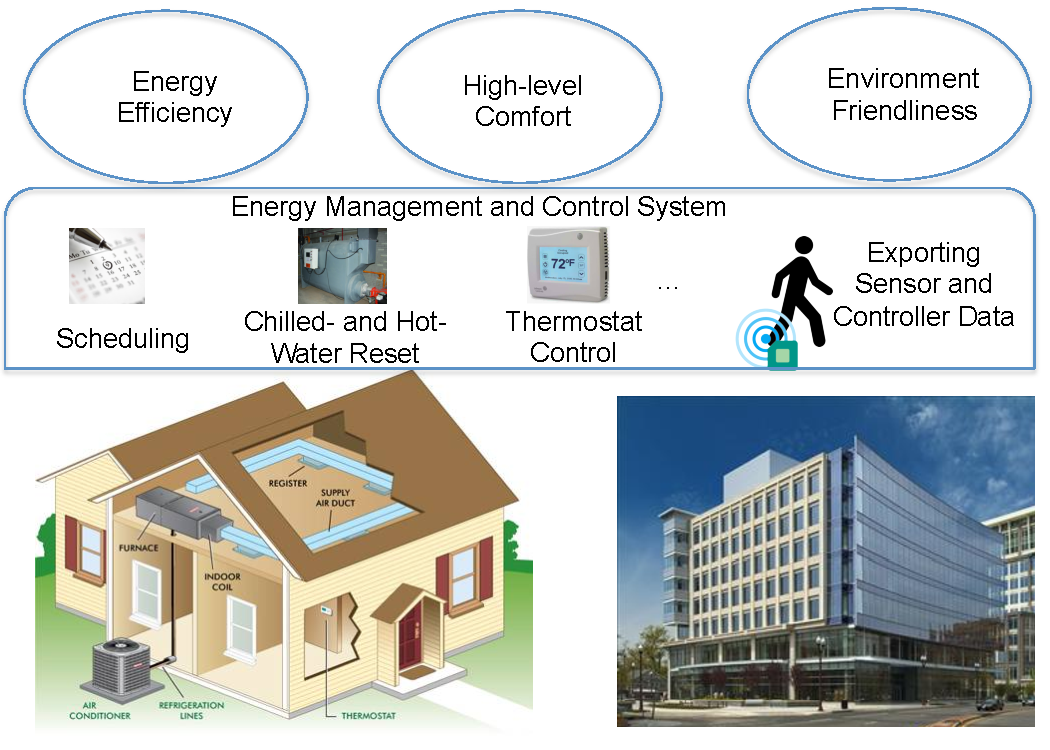
\includegraphics[width=0.8\textwidth]{fig/smartbuilding.pdf}
\caption{Smart Buildings Schema.\label{fig_smartbuilding}}
\end{figure}

%One such application is in \emph{urban computing}, primarily from the perspective of data science. 
%A data scientist role has become critical in being able to learn, process, analyze, and deliver actionable insights that can help realize the promises of this \emph{unprecedented urbanization}. 

\subsection{Challenges in Smart Building Research}
Smart building aims to achieve significant energy saving by utilizing advanced energy technology. 
The intelligent energy management system monitors devices, controls appliances and conserves energy. To design an energy-saving building, we need to conduct several procedures to achieve this goal. Each change to existing procedures faces different problems. 
\begin{itemize}
  \item Collecting data. 
Determining how to collect accurate energy data using state-of-the-art technology is a fundamental problem. 
  With the advent of sensor technology, wireless sensor nodes and active RFID tags are 
  installed on devices or worn by people to gather comprehensive information \cite{vullers2010energy}. 
Generally, energy consumption, water usage, gas expenditure, air temperature or noise status are monitored by meters or wireless sensors, then the collected data is transmitted to the computer and to storage. 
Identifying how to measure and collect this data precisely with low cost and minimal intrusion has always been a problem. 
  \item Quantify opportunities.
 Analyzing data and discovering opportunities for energy optimization are another concern. 
First we need to identify the devices which consume a large amount of power or water or gas, when they are operated, and the regular patterns of energy consumption. Next, we need to figure out the possible opportunities to decrease energy consumption by evaluating the usage time and energy cost. 
\item Target and Schedule. 
Determining how to set  a reachable target by scheduling the devices inside the building is an optimization subject. When to turn devices on or off, how to set the temperature inside the building without sacrificing the comfort of people, and how to make rules for device automation have been popular research problems. 
\item Track progress.
To evaluate whether a scheduling plan is effective is an important issue. 
How to introduce new technology and update models in time is a challenge. 
%New updated models or technology could be introduced to optimize the energy usage. 
\end{itemize} 

In this work, we focus on quantifying opportunities in energy management. Other issues, such as how to collect energy consumption data, how to schedule the electrical devices or other water use ends, and how to refurbish models to optimize energy usage, are outside the scope of this work. 

%We study two issues in smart buildings research, such as quantify the energy usage of each device with non-intrusive approach (energy disaggregation), occupancy prediction with monitoring sensor of people, which can provide suggestions on the daily plan of heating, ventilation and air conditioning (HVAC) system. 

\subsection{Goals of this Work}
In this work, we endeavor to clarify the problems of how to qualify energy usage inside buildings. Then we implement existing approaches or enhance current methods to pinpoint energy usage as accurately as possible. This introductory section describes the research motivations, then explains our data-driven models for energy measurement, and concludes with a list of our contributions to smart building research. 

\textbf{Research motivation}

\emph{Analytics} has transformed the perception of the world we live in. Big Data is the lingua franca of the twenty-first century, and data science has become an essential lens through which decision making is seen. The massive amounts of data collected via several active and passive instrumentations positions us truly in an \emph{age of information}. Data via Web 2.0, social media, the internet of things, traffic flow, gene sequencing, etc., in conjunction with the advancement of using data-mining and machine-learning to glean actionable insights, have influenced the world in designing policy, pricing products, launching political campaigns, and many other applications. The power of \emph{data analytics}, thus, is in its diversity. 
With respect to energy quantification, we introduce data-driven models to address several problems that we study in this thesis. 

\textbf{Topic 1: Disaggregation to energy}

While people generally agree on the importance of conservation and
usage curtailment, they often find it difficult to quantify 
{\em where, when} and {\em how much} electricity is consumed.
Typically, residences and businesses receive
monthly electricity bills indicating aggregate usage, with no information on
the breakdown of consumption by appliance/device, time of day, or day of
week (this is an area in great flux, however). Research has 
shown that simply making such feedback available to users
can reduce consumption by up to 50\%, although typical saving 
are in the 9\% to 20\% range \cite{book2014us}.%\cite{energydatabook2011}.

One obvious approach to determining the breakdown of consumption is to install
power meters in every circuit (and sub-circuit)
to capture the consumption of individual devices in homes and
offices. Such installation is costly and intrusive, making 
this option non-viable in practice. 
An alternate
solution, called energy disaggregation or non-intrusive load monitoring
(NILM),
first proposed by Hart~\cite{hart1992}, is using analytics to 
{\em infer} the breakdown of consumption from an aggregate 
power measurement of a
site. This drastically reduces the number of meters required per 
home/installation, typically to just one meter. Furthermore, depending on the analytics desired, it is possible to
use the measurements already being recorded by a utility meter for
disaggregation, especially in cases where utility companies have deployed
smart meters.
Energy disaggregation is hence today a booming area both offering
challenging problems for data analytics and having practical relevance in a
number of areas including sensor networks and building analytics.

%Water disaggregation \cite{carboni2016contextualising} is similar to electricity disaggregation. 
%By measuring the water flow rate, vibration or pressure in the hot and cold water, 
%the flow trace of each water use end is inferred. 
%This breakdown process is somewhat different from the electricity disaggregation 
%because of the characteristics of water use ends. 

\textbf{Topic 2: Occupancy Prediction}

An effective approach to save energy in homes is to 
efficiently use electric devices.  
In residential buildings, 
the biggest consumer of electricity is the HVAC 
(heating, ventilation, and air conditioning) system, which generally accounts for ~54\% 
of the building's electricity consumption~\cite{book2014us}. 
Determining how to automatically start up and shut down the HVAC unit 
is thus a key problem. 
One solution is to predict the occupancy of a home by analyzing the activities of daily life 
inside the building. 
Based on the occupancy information, 
an automatic control system can then be installed
to operate the HVAC. 

\subsection{Temporal Data Mining and the Probabilistic Model}
Temporal datasets display a character of time-dependency. 
They are recorded frequently in smart buildings 
and build scenarios to infer the energy usage of people.
 Temporal data mining revolves around the techniques (algorithms) that enumerate structures, patterns, and signatures over temporal data (time series, for instance). 
 A survey \cite{laxman2006survey} has investigated several efficient 
 techniques to discover the patterns in ordered data streams.  
 The techniques used to discover significant patterns vary according to the dataset. 
 One of the compelling patterns in temporal data mining is frequent episodes \cite{mannila1997discovery}.

\textbf{Frequent Episode Discovery}

Frequent episode discovery is proposed in \cite{mannila1997discovery}. 
Given a sequence of events $<(E_1, t_1), ..., (E_n, t_n)>$, 
where $E_i$ denotes the $i^{th}$ event at the time of $t_i$, 
the aim is to find temporal patterns (called \textit{episodes}) that occur 
frequently in the long sequence. 
This episode is an ordered event collections. 
For in-stance an episode $(A\rightarrow B\rightarrow C)$ represents that event type $A$ comes before event type $B$, 
which occurs before event type $C$. 
The occurring time of these events are unnecessary to be consequent. 
The frequency threshold is decided by a user. 
 Several data mining algorithms have been researched to 
 discover the frequent episodes \cite{mannila1997discovery, laxman2005discovering}.
 
\textbf{Motif Mining in Multi-variate Time Series Data}

Motif mining is a temporal data mining technique that was initially proposed in ~\cite{motif1} and \cite{motif2} and extensively studied in \cite{minnen2007improving, tanaka2005discovery, motifgoal}. The fundamental idea behind \emph{motif mining} is that it symbolically encodes the numerical time series data. After this encoding, the symbols combine to form episodes in the data, resulting in patterns that can be mined. Furthermore, by combining domain-specific information and pattern mining techniques, we extract frequent,  meaningful episodes from the symbolized time series.

Furthermore, when there are time series that describe the data, we employ \emph{multi-variate motif mining} to find meaningful patterns. The algorithms for multi-variate temporal motif mining are similar to the univariate case, except that the symbolic encoding is represented as a vector. Therefore each time point in the data is represented as a vector of symbols, with each symbol corresponding to one of the several time series that represents the data. Now, the combination of these vector symbols forms episodes that can be mined from the multi-variate time series data. Again, by combining domain specific knowledge, we extract meaningful episodes from the data.

\textbf{Episode Generating Hidden Markov Model (EGH)} 

A hidden Markov model is a ubiquitous construct to model time series data. It is used to represent probability distributions over a sequence of data. The hidden Markov model gets its name from two important properties. The observation (data point) is generated by a process whose state is \emph{hidden} from the observer. Second, the state of this hidden process satisfies the \emph{Markov} property that the current state is independent of all prior states. The \emph{Episode Generating HMM}, researched in \cite{laxman2005discovering}, connects the episodes with an HMM model and has a parameter to evaluate whether an episode is frequent or not. A mixture of EGH describes a situation in which several frequent episodes are embedded into a time series, and can be used to predict whether a target symbol will be the next symbol in a time series.

\textbf{Applications of Motif Mining and EGH}

In our work we apply motif mining techniques, both univariate and multivariate cases, to energy disaggregation. By correlating episodic information with the switching on and off of appliances from time-series represented energy data, we are able to successfully determine the one-to-one mapping between a certain appliance and its usage patterns and time. 

\begin{figure}[!hbtp]
%\makebox[\textwidth]{\framebox[5cm]{\rule{0pt}{5cm}}}
\centering
\includegraphics[width=0.7\textwidth]{fig/framework.pdf}
\caption{Overall Framework for Smart Building Issues.\label{fig_framework_whole}}
\end{figure}

Figure \ref{fig_framework_whole} gives a overall framework on the issues of the above smart building issues. 
By mainly collecting the energy consumption of profiles of electrical devices, %or water use ends, 
and the activities of daily life profiles of people inside buildings, we analyze the frequent episodes from these profiles with temporal mining and probabilistic models. Based on this analysis, a controlling and scheduling system can be developed to control individual devices. 

The formulation of the EGH model lends itself to predicting occupancy in a residence or any building. We develop an EGH model based on occupancy prediction that can assist in automated turning on or off of the HVAC system, which can single-handedly reduce a good portion of the energy consumption footprint. We demonstrate that our algorithm can effectively forecast occupancy.  

\textbf{Contributions}

In this work we make efforts to resolve some of the problems arising in smart building research with 
temporal mining approaches.
\begin{enumerate}
	\item The episode mining approach works effectively for discovering significant patterns in the problems of energy disaggregation and occupancy prediction. 
	\item We extend previous temporal mining approach~\cite{shao2013temporal} to a multivariate piecewise motif mining algorithm for energy disaggregation. 
	\item The episode-based model Episode Generating HMM (EGH) and a mixture of EGHs performs well for event prediction in occupancy prediction. 
\end{enumerate}

\section{Prior Work}
Electricity disaggregation uses the electricity consumption level at the main entry into a building or house 
to infer whether a device inside the building is on or off. 
The features used include initial real power and reactive power~\cite{hart1992} from a dataset which is recorded in 
a low-frequency range. 
With advances in electrical meter technology and the availability of less expensive meters, 
more and more features are being extracted from the high-frequency data set and used for disaggregation, such as 
the transient state generated when a device turns on or off~\cite{shaw2000PhdThesis},
the raw current waveform~\cite{srinivasan2006neural}, the voltage waveform~\cite{lam2007novel}, 
the transform of the current waveform~\cite{chan2000harmonics}, 
and harmonics of non-linear devices~\cite{chan2000harmonics}. 
Even on-AC power features such as power line noises~\cite{patel2007flick}
are exploited jointly with AC power features like  
time of day, and device correlations~\cite{kim2011unsupervised}
in modern systems.
Increasingly,  
research is being focused on unsupervised learning and semi-supervised learning algorithms because  
these algorithms do not require the power consumption of 
each device,   
and the power of individual devices are very difficult to obtain. 
It is only in
 the last few years that 
unsupervised learning algorithms
have been used, including
hierarchical clustering~\cite{gonccalves2011unsupervised},
factorial hidden Markov models (FHMMs)~\cite{kim2011unsupervised},
additive factorial approximate MAPs (AFAMAP)~\cite{kolter2012aistat}, 
difference FHMMs~\cite{parson2012nonintrusive}, 
and motif mining~\cite{shao2013temporal}.
Semi-supervised learning 
algorithms~\cite{lam2007novel,johnson2012bayesian} have also
been proposed.
In this paper, we assume the number of devices 
and the number of power level states of each device 
are known. Hence, we formalize the disaggregation 
as a semi-supervised problem and 
provide solutions to the following three challenging problems.
\begin{enumerate}
\item Several devices may have the same real power, and
it is difficult to distinguish these devices using only the recorded aggregated
power time stamp.
\item Many devices may turn on or off at the same time.
\item Instead of having a discrete range of power
levels, there are devices whose power consumption levels
   vary gradually, e.g.,
  variable speed devices (VSD) and lights with dimmers.
Once their power usage is aggregated with that from other devices,
disaggregation becomes increasingly difficult.
\end{enumerate}
Since obtaining a low-frequency dataset is more practical in real buildings, 
we focus mainly on real power, which can be easily extracted 
from a low-frequency dataset.  
%Water use disaggregation has emerged in recent years, and so far 
%the applied algorithms are 
%limited to supervised learning algorithms~\cite{carboni2016contextualising}. 
%This chapter proposes water disaggregation as a semi-supervised learning algorithm 
%by presuming that we know the number of water use ends and the water usage level of each 
%water user end.  

%% prior work for occupancy prediction
Accurately predicting whether a home is occupied is a difficult task. 
People in the same home have different daily schedules; 
some go to work and others stay at home for a period of time.  
A great deal of research has been done to track the activities of people 
to infer the home occupancy. 
Researchers have made efforts to collect data by sensors, smart phones, 
the calendar, and weather information. 
Most of the approaches that model and predict occupancy primarily use sensor data to detect conditions 
such as room occupancy, use of electrical appliances, water usage, etc.
Several supervised learning approaches, such as kNN, neural networks, rule-based models, 
and Markov chain models have been used to model and predict building occupancy 
\cite{scott2011preheat,alrazgan2011learning,mahmoud2013behavioural,erickson2010occupancy,beltran2014optimal}.  
Using the kNN supervised learning algorithm and monitoring sensor data 
for a portion of the day, 
Scott et al. predict an entire day's occupancy in~\cite{scott2011preheat}. 
A neural network approach using a binary time series based on 
occupancy/unoccupancy along with exogenous input network (NARX) is 
proposed in \cite{mahmoud2013behavioural}. 
Mahmoud et al. tackle the problem by presenting a non-linear autoregressive 
model with an exogenous input (NARX) network. 
Several Markov chain models, like the blended Markov chain, 
closest distance Markov chain, 
and moving-window Markov chains are presented in \cite{erickson2010occupancy}. 
A mixture of multi-lag Markov chains was used to predict the occupancy of 
single-person offices \cite{manna2013learning}. 
In that work, the authors also compare their model with the Input Output Hidden Markov Model, 
First Order Markov Chain and the NARX neural network. 

A recent survey~\cite{kleiminger2014predicting} compares major occupancy 
predictions algorithms against the LDCC dataset~\cite{kiukkonen2010towards}, which was collected by 
GPS and other sensors. 
It shows that time-based presence probability~\cite{krumm2011learning} performs slightly better than the preheat kNN approach~\cite{scott2011preheat}. 
Since the preheat kNN approach~\cite{scott2011preheat} is more widely applicable,  
in that it can be used against both GPS and sensor datasets, 
we set it as a baseline method for comparison. 

%%%%%comment several paragraphs
\iffalse
These superseded learning approaches are classified into several categories. 
The first is on the probability density distribution of key events. 
\cite{tominaga2012unified} proposes that at a time,  a person goes out has a Bernoulli distribution. 
The second effective benchmark approach is kNN. 
kNN approach is employed in 
\cite{scott2011preheat} to predict the occupancy of the left day 
after knowing the occupancy in the partial day. 
It splits the whole day's time into 96 15-minutes intervals 
then to find the top-5 similar day in the training date. 
The average of these similarity is the predictive occupancy. 
The third is the pattern discovery by rule and neural network. 
A rule-based approach is proposed by
\cite{alrazgan2011learning}  for occupancy prediction under the frame work of Decision Guidance Query Language (DGQL). 
A variant of neural network has been proposed by 
\cite{mahmoud2010occupancy}. \cite{mahmoud2010occupancy} converts the data into binary occupancy/unoccupancy data in the first step. Then a model name non-linear autoregressive network with exogenous input (NARX) network is modeled for prediction. 
\cite{mahmoud2013behavioural} also uses binary time series with NARX network. 
The last are models related to Markov chains. 
Several Markov Chains have been compared in the paper of \cite{erickson2014occupancy}, including blended Markov Chain, closest distance Markov Chain, and the moving window Markov Chain with respect to modeling occupancy. 
\cite{erickson2010occupancy} uses moving-window markov chain for occupancy prediction. 
\cite{erickson2013poem} utilizes the markov chain model and blend markov chain model for prediction. 
\cite{beltran2014optimal} uses a blend-markov chain model for prediction. 
\cite{manna2013learning} uses mixture of multi-lag markov chains to predict the occupancy in single person offices. It compares with other previous approaches Input Output Hidden Markov Model, First order Markov Chain and NARX Neural Network. 

This paper contributes the follows:
1) formulate the problem as a temporal mining problem;
2) mine the activity patterns according to time and gap;
3) the occupancy prediction performance of this temporal mining approach works better than kNN for most cases.
\fi

%\section{Multivariate Motif Mining to Disaggregation}
With the advent of modern sensor technologies, 
significant opportunities have emerged to help conserve energy in 
residential and commercial buildings. Moreover, the rapid \emph{urbanization} we are witnessing requires optimized energy distribution. 
Energy disaggregation attempts to 
separate the energy usage 
of each circuit or each electric device in a building 
using only aggregate electricity usage information from 
the whole house meter. 
Usually two-phase or three-phase electric power is 
connected to residential and commercial buildings. 
%Similarly, water disaggregation aims to discover each 
%water use end by only knowing the 
%hot and cold water usage from the whole house water meter.
We tackle energy disaggregation as a multiple-phase data disaggregation problem. 
The aim of this section is to identify electrical devices from 
two phases of aggregated data. 
Unlike previous work which disaggregate devices
from the sum of multiple phases, 
the time series information from each phase and the correlation of a device between/among phases 
are fully used.  
All of this information enables us to characterize more devices. 

%This work makes the following contributions in the field of disaggregation:
%\begin{enumerate}
%\item It can disaggregate aggregate data from multiple phases.
%\item It can separate the continuously variable loads which are mixed in electricity. 
%\item This approach can be used for both electricity disaggregation and water disaggregation.
%\end{enumerate}

\subsection{Disaggregation Formalism}
We propose a semi-supervised approach for disaggregation; i.e.
We assume that we know the on and off events for a short period of time for all devices, %or water end uses, 
and use that information to deduce the power levels, %or water usage, 
or to obtain the startup vectors of every device.

For our purposes, we define the disaggregation problem as follows:
Given $K$-phase aggregated power 
%or $K$ aggregated water consumption time series 
$Y_k=y_1^{(k)}, ..., y_T^{(k)}$, and a set of
power %or water related 
and contextual features, $f=f_1, ..., f_T$ over a period of time T, 
the problem is to estimate the disaggregated power %or water consumption 
of $M$ devices 
$\hat{X_m }= \hat{x}_{1}^{(m)}, ...\hat{x}_{t}^{(m)}, ... \hat{x}_{T}^{(m)}, m\in[1, M]$, 
such that a loss function of the sum of the power %or water consumption 
of the $M$
devices and the sum of the $K$ phases of aggregated power %or water consumption 
is minimized. 
\begin{equation}
\label{eq_powerObj}
\min_{\hat{x}_{t}^{(m)}} \{ \sum_{t=1}^T \mathscr{L}_t(\sum_{m=1}^M \hat{x}_{t}^{(m)}, \sum_{k=1}^Ky_t^{(k)}) \},
\end{equation}
where $\mathscr{L}_t$ is the loss function between 
the sum of $M$ estimated time series at $t$, 
and $y_t^{(k)}$ is the ground truth phase $k$ aggregated power %or water 
feature at time $t$. 
$\mathscr{L}$ is usually the $\mathscr{L}1$-norm $|\sum_{m=1}^M \hat{x}_{t}^{(m)} -\sum_{k=1}^K y_t^{(k)}|$
or the $\mathscr{L}2$-norm $(\sum_{m=1}^M \hat{x}_{t}^{(m)}-\sum_{k=1}^Ky_t^{(k)})^2$.

\subsection{Recursive Multivariate Piecewise Motif Mining}
To solve the problem of separating a multi-dimensional time series into several time series, 
I propose the approach of recursive multivariate piecewise motif mining. 
Motif mining has been well studied in previous work \cite{motif1} and \cite{motif2}. 
Multivariate or multidimensional motif mining is further extended in \cite{minnen2007improving} and \cite{tanaka2005discovery} and \cite{motifgoal}. 

Motif mining is applied to energy disaggregation in \cite{shao2013temporal}, 
in which discrete on/off events are exploited. 
This research enhances previous work by piecewise motif mining, 
where the on/off event is comprised of several consecutive data points, 
i.e. piecewise, other than individual discrete one.
Also, I use multivariate motif mining to make full use of two- or three-phase aggregated data. 

The framework of recursive multivariate piecewise motif mining to energy disaggregation is illustrated in Figure \ref{fig_multivariateMotifming}. 
The input includes multiple-phase aggregated data, such as two-phase data Mains1 and Mains2, 
and the power levels of each device. 
During the whole procedure, I recursively apply piecewise motif mining to two-phases and single phase diffs data.
The first step is to identify electrical devices which draw power from both phases.
Generally these devices consume a large amount of power, such as the water heater indicated by the blue line.
These devices draw equal power or disparate power from both phases synchronously. 
%draws equal power from both phases. 
%By comparing the diffs of these two phases, 
%we discover the same power changes during the on/off events. 
%With multivariate motif mining, 
%we can identify these large power consumption devices. 
Secondly, I remove the power consumption of the devices which draw power from both phases.
This action decreases the noise interference caused by large power consumption 
and increases the possibility to disaggregate more devices with low-power consumption. 
Then we apply piecewise motif mining to single-phase data to separate 
the devices that draw power only from that phase, 
such as the humidifier indicated by the green line. 
\input{multidisaggfig/multivariateMotifmining}
Generally, multivariate piecewise motif mining is divided into four steps, as shown in Figure \ref{fig_multivariatePiecewiseMotifMining}.
Step 1 is to search for piecewise events from the two-phase or three-phase data.
Step 2 is to encode events from multiple phases. 
Step 3 aims to mine frequent motifs from the encoded events list.
The last step targets to recover devices from mined motifs. 
\begin{figure}[h]
\centering
\includegraphics[width=0.7\textwidth]{multidisaggfig/multivariatePiecewiseMotifMining.pdf}
\caption{Multivariate Piecewise Motif Mining.}
\label{fig_multivariatePiecewiseMotifMining}
\end{figure}

\subsubsection{Piecewise Motif Mining}
Motif mining aims to uncover the repetitive patterns in time series data, and works best for discrete events. Piecewise motif mining is proposed 
for energy disaggregation to detect on/off events. 

\begin{definition}{\textbf{Piecewise Event}}
Given a time series diffs data $y_1, ...., y_{n'}$, where $\forall$ $|y_i| < \eta$. 
A piecewise event is the sum of these $n'$ number of diffs data, $e= \sum_{i=1}^{n'} y_i$. 
\end{definition}
Each piecewise event corresponds to an on/off event of an electric device. 
The value of $\eta$ is the noise range of each device, 
which is usually less than the 10\% of $|e|$.  

\textbf{Piecewise Events Search from Multiple Phases} \\
The majority of electrical devices which draw power from multiple phases consume larger amounts of power than electrical devices which connect to single phase. 
To disaggregate such a device, we need to 
discover specific on/off events features to separate them. 
%on/off events which are yielded by this single device from two-phase or three-phase aggregated data. 
Generally such an electrical device draws power from multiple phases synchronously 
and constructs a  pattern. 
Some devices may consume equal power from both phases all the time,  and so their power consumption patterns from both phases keep the same.
Other devices may show different power usage patterns when drawing power from two phases. 
%The power consumption from both phases may be exactly synchronized and keep the same all the time. 
%Either, the power consumption drawn from a single device differs much. 
\input{multidisaggalg/synchronizeEvents}
Algorithm~\ref{alg_synchronizeEvents} describes how synchronized events from two phases are revealed.  
This input include the two-phase aggregated diffs data and big power consumption threshold $\theta$. 
This threshold guarantees we only discover big power consumption devices. 
We review the phase-1 diffs data. 
If any absolute value $|y_i^{(1)}|$ is greater than $\theta$, 
both previous and posterior five diffs data points from time $i$ are checked. 
For these 10 points values, 
at each time $j$, if the difference between phase-1 $y_i^{(1)}$ and phase-2 $y_i^{(2)}$ is in the range of $0.2*|y_i^{(1)}|$,  
we assert that the diffs data points from these two phases are relatively the same and synchronized. 
The synchronization implies that 
these two identical amounts power consumption comes from a single device. 
Therefore we sum the synchronized power level diffs data and compute the power consumption at time $i$ as $e_i$.  
When $e_i>0$ that denotes an on event, and $e_i<0$ means an off event for a certain device.

Next we transfer these two-phase diffs data into 
an ordered on/off event list $e_1, ..., e_{n'}$,
then we apply motif mining to this events list. 
By matching the devices which consume power greater than $2*\theta$, 
we can separate all devices which draw equal amount of power from two phases.  
%Since we already know the power levels of each device, 
%we just choose those devices which include power levels bigger than $2*\theta$. 
%By applying motif mining, 
%we can separate all devices which consume two-phase power greater than $\theta$ equally. 
%For dataset Study10, we set $\theta=500W$. 
%This approach helps us to discover two devices waterHeater2 and heatingIndoor. 
%All of the on/off events of these two devices are found out. 

\subsubsection{Encoding Events From Multiple Phases}
After deleting all the synchronized events from phase-1 and phase-2, 
we apply multivariate piecewise motif mining to the remaining phase-1 and phase-2 diffs data, 
to detect devices which consume large amounts of power 
and draw power from two phases synchronously yet unequally. 
There are different power drawing patterns from these two phases.  
We encode these two-phase diffs data, which occur at the same time, as a new event $e$. 
Figure \ref{fig_eventEncoding} gives an example of how the events from two-phase circuits
are encoded. 
We extract an event which consumes power greater than $\theta$, 
then we check five more data points before and after it. 
The values of the 11 data points relevant to this event in Main1.diff are [0, 0, -18, 18, 1093, 1830, -196, -68, -37, -36, 0]. 
The concurrent events listed in Main2.diff are [0, 0, 0, 18, 9, 1946, 440, -51,-36,-36,0]. 
Since the events at the peak occur in the two phases as $(1830, 1946)$, 
and the difference of these two powers $1946-1830=116$ is in the $0.2*1830$ range, 
we consider that these two changes may come from a single device. 
When looking for insight into these two vectors, 
we observe that the sum of the changes of phase 1 is 2604W, and the sum of the changes of phase 2 is 2290W. 
They are in the same range, i.e. $2604*0.8 < 2290$. 
Therefore, we declare that the power changes from these two phases definitely come from a single device. 
We select two of these values and encode them as $e_{1'}=(1093, 9)$, $e_{2'}= (1830, 1946)$
\begin{figure}[h]
\centering
\includegraphics[width=0.5\textwidth]{multidisaggfig/synchronizeDifferentEventEncoding.pdf}
\caption{Encoding Events from Multiple Phases.}
\label{fig_eventEncoding}
\end{figure}

The piecewise events for this single device are $e= [e_{1'}, e_{2'}]$. 
Applying frequent motif mining, 
we separate this large power consumption device which draw power from two phases unequally. 





\section{Constraint Motif Mining and EGH for Prediction}
Modeling activity of daily life (ADL) has become a burgeoning research topic, 
since people demand a comfortable life at home
at a lower cost. 
Since heating and cooling spaces consumes $\sim$53\% of the total electrical usage 
by heating and cooling spaces %\cite{energydatabook2011} 
of an average household, 
automating the operation of HVAC devices to save energy is important. 
One of the crucial components required to achieve this goal is 
to model and predict the occupancy of a home. 
Supervised learning approaches on the analysis of indoor temperature~\cite{kleiminger2014predicting}, 
smart phones' GPS data~\cite{koehler2013therml}, 
electricity consumption~\cite{erickson2010occupancy} and 
sensor data by tracking indoor activities~\cite{scott2011preheat,alrazgan2011learning} 
are effective ways to approach this prediction problem. 
Prediction of occupancy using sensor data has been broadly researched. 
By capturing daily activities, like room occupancy of the house, 
usage of electrical devices, 
and usage of water systems using sensors, 
researchers have modeled occupancy~\cite{mahmoud2013behavioural,erickson2010occupancy,beltran2014optimal} 
and used these results to automate the control of the HVAC system. 

Although the supervised learning kNN~\cite{scott2011preheat}, 
neural network~\cite{mahmoud2013behavioural} and Markov model~\cite{erickson2010occupancy} 
are effective, 
the detailed household activities represented as a time series are not fully utilized. 
Daily activities such as waking up, cooking, washing, and commuting to work/school and back 
have different patterns based on the day. 
For instance, the schedule on a working day is significantly different from that of a weekend 
or a holiday. 
Thus, this scenario leads itself to episode mining analysis, 
which can be used to predict household occupancy. 
Using this strategy of episode mining for occupancy prediction has three advantages. 
First, episode mining, a temporal mining approach, mines according to the time 
distribution for each type of activity. 
Second, it builds the activity scenario and connects the episode with 
a probabilistic hidden Markov model (HMM). 
Unlike previous models, 
the time and order of each kind of activity are fully utilized. 
Third, the algorithm predicts according to the scenario-based probabilistic model episode 
generative HMM (EGH). The prediction accuracy is better than the existing models. 

%This work's contributions can be highlighted in the form of the three questions below. 
%\begin{enumerate}
%\item How can we mine for meaningful scenarios? 
%Episode mining can mine many frequent episodes, but not all the episodes are useful 
%for occupancy prediction. 
%By narrowing the episodes according to the start state, 
%end time, event dwelling time and the gap between two activities, 
%we can interpret these episodes and provide insight as to 
%which episodes are informative. 
%\item How can we predict the occupancy more accurately?
%Our dataset comprises detailed information of the various activities of a household 
%tracked as a time series on a daily basis. 
%Thus our episodes have rich detailed information based on occupancy and 
%unoccupancy of the household. 
%Since we are mining episodes from this data, 
%the accuracy of occupancy prediction improves significantly. 
%\item  Can it help save electric usage at home?
%The prediction occurs at least 15 minutes ahead of a person 
%leaving or coming back. 
%By connecting this prediction result to an automatic HVAC controlling system, the HVAC can be turned on or off  ahead of the occupancy change. 
%Since the HVAC does not work during occupancy, 
%this saves electric usage. 
%\end{enumerate}

\subsection{Occupancy Prediction Problem Formulation}
Given $M$ time series, 
each time series $X^{(m)}=X^{(m)}_1, ..., X^{(m)}_t, ..., X_T^{(m)}$ 
represents a sequence of room occupancy of person $m$ inside 
a home over $K$ days, 
where $X_t\in s$ denotes that $X$ belongs to a finite room set $s$ at the sequence number of $t$, 
and $m\in\{1,...,M\}$. 
%Each $X$ is has a start time $X.start$ and an end time $X.end$.  
Let $Z$ denote that the home is unoccupied and $Z\in s$.  %$Z=0$ if a house is unoccupied; $Z=1$ if the house is occupied.  
%Its meaning equals to certain symbols from set $s$. 
We predict whether person $m$ stays at home the rest of a day from time $T$,  i.e. during $T+1$, $T+2$, ..., $\Delta T$, 
 
\begin{equation}
\hat{Y}^{(m)}=\hat{Y}_{T+1}^{(m)},...,\hat{Y}^{(m)}_{T+\Delta T}
\end{equation}
where $Y_{T+\Delta t }^{(m)}=Z$ if person $m$ does not stay at home at time $T+\Delta t $;
otherwise, $Y_{T+\Delta t}^{(m)} \neq Z$. 
%The un-occupancy of the whole house is the intersection of un-occupancy of all people. 
If any person $m$ stays at home $Y_{T+\Delta t}^{(m)} \neq Z$, then this house is occupied $Y_{T+ \Delta t} \neq Z$. 


\subsection{Temporal Mining Mixture Model}
We use a three-pronged approach to tackle the problem of mining and predicting unoccupancy, as 
shown in Figure~\ref{fig_framework}.
\begin{figure}[h]
\centering
\includegraphics[width=0.5\textwidth]{adlfigs/framework.pdf}
\caption{Occupancy Prediction Framework.\label{fig_framework}}
\end{figure}
Given indoor activities time series of a person over a period of time, 
first, we use an episode mining algorithm to discover frequent episodes from the past days' data. Then we connect each episode with an EGH and build a mixture EGH model. 
Based on the mixture model, we predict when each person will leave and come back the house. 
If all people leave, then the house is unoccupied. 

%Before formalizing the problem statement, we introduce several concepts and notations. 

\textit{Episode} 
An episode is a collection of ordered events. 
Here an episode refers to an ordered events which are 
highly relevant to the occupancy status inside a building. 
For instance, we represent 'S' as sleep, 
'K' as kitchen, and 'Z' as going out. 
If an episode $S \rightarrow K \rightarrow Z$ is found, 
the story is described as a person getting up, 
going to the kitchen for breakfast, and then leaving the house. 
An episode $\alpha$ is composed 
of a series of ordered events
$\alpha=\langle X_1,..,X_t,...X_T \rangle$, 
where $X_t$ denotes that $X$ occurs at a sequence of $t$.  
The event $X_t$ may be the point event or dwelling event. 
The dwelling event
has a start time $X.start$ and end time $X.end$. 
In this paper  $X$ denotes a dwelling event and 
represents which room a person stays 
inside a building, i.e., this building is \emph{occupied}. 
Since $Z$ denotes a room is unoccupied, 
$Z.start$ is the point at which a person or all people inside the building leave, and 
$Z.end$ is the point at which a person or all people come back. 

%\textit{EGH} Episode generative HMM model is a 
%type of HMM model which connects each episode $\alpha$ 
%with a special HMM model $\Lambda_\alpha$. 
%The uniqueness of the EGH is that 
%the transition matrix and 
%emission matrix is only decided by a noise parameter $\eta$. 
%The value of $\eta$ is computed based on the frequency of the 
%corresponding episode $\alpha$. 

\subsection{Time-gap Constraint Episode Mining}
\textbf{Episode Mining}
Episode mining has been studied in previous research \cite{mannila1997discovery}. 
It uses a non-overlap mining approach to find the frequent episodes. 
Episode mining has been applied to energy disaggregation to help conserve energy in buildings~\cite{shao2013temporal} in sustainability research. 
In contrast with previous research, 
the events in this application of occupancy prediction 
dwell at an event for a period of time. 
As a result, we extend the above two 
episode mining algorithms~\cite{laxman2008stream,patnaik2008inferring} 
and enforce more constraints.
One change is to 
adopt right alignment for the first element in the episode mining. 
%In the example of $AB$, 
%the mined second instances is $\langle A_9,B_{11} \rangle$. 
The second modification is to 
add time constraints and 
apply gap duration constraints between 
two consecutive events inside an episode. 
%Figure \ref{fig_durationgapconstraint} shows an example of time-gap constraint episode. 
%\begin{figure}[h]
\centering
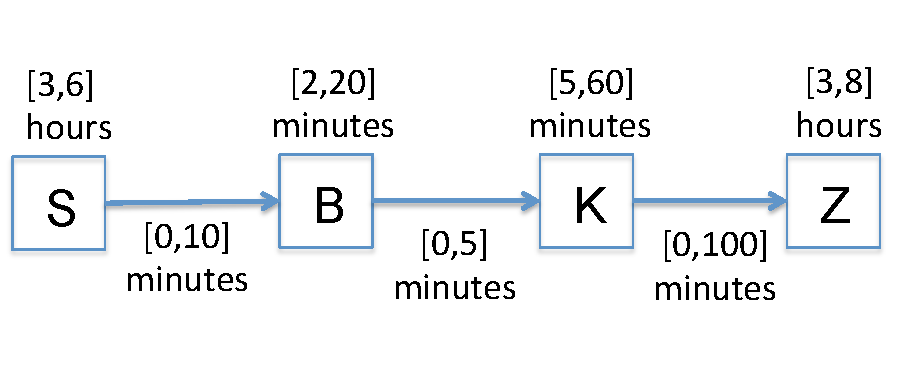
\includegraphics[width=0.5\textwidth]{adlfigs/durationgapconstraint.pdf}
\caption{Example of Duration-gap Constraint Episode.\label{fig_durationgapconstraint}}
\end{figure}

\begin{figure}[!hbtp]
\centering
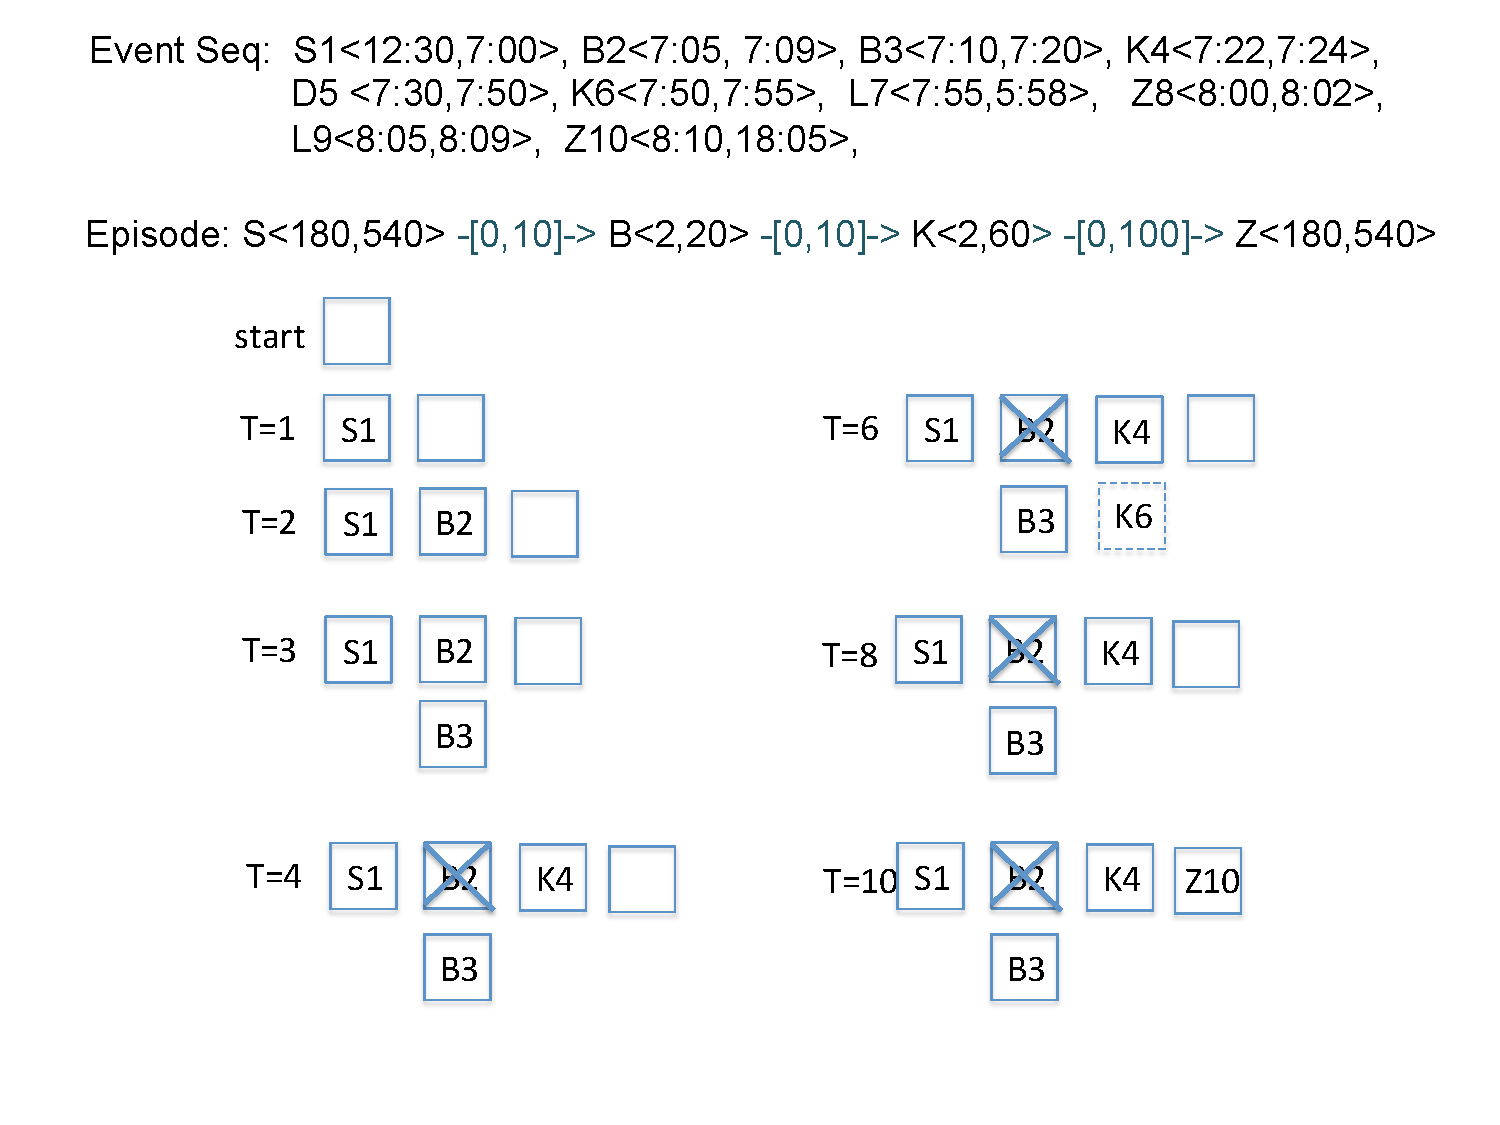
\includegraphics[width=0.5\textwidth]{adlfigs/MingExample.pdf}
\caption{Time-gap constraint episode mining example.\label{fig_MingExample}}
\end{figure}

Figure~\ref{fig_MingExample} shows a time-gap constraint episode mining example. 
Let us assume we have a frequent episode $S\rightarrow B \rightarrow K\rightarrow Z$. 
We then add the time constraints to each event $\{S,B,K,Z\}$. 
The dwelling duration of $S$ is 3 to 6 hours,   
of $B$ is 2 to 20 minutes, 
of $K$ is 5 to 60 minutes, 
and of $Z$ is 3-9 hours. 
In addition, we set gap duration between any two consecutive events. 
The gap duration of $SB$ is calculated as $\Delta{SB} = B.start-S.end$. 
We set the maximal gap time between SB, BK, and KZ as 
10 minutes, 40 minutes and 100 minutes; 
the minimal gap time is 0. 
Then we have a stream composed of the sequence of dwelling events "Event seq," as shown 
in Figure~\ref{fig_MingExample}.  
 The time-gap constraint episode mining process 
 to discover a frequent episode uses the following method. 
 Let the $node$ structure denotes each element in any episode,  
as depicted as a square box in Figure~\ref{fig_MingExample}.  
Let $waits$ refer to a structure which pairs with an episode 
and has the same length of this episode. 
Initially, a $waits$ structure related to episode $S\rightarrow B \rightarrow K\rightarrow Z$ is created. 
A $node$ structure related to $S$ is created 
and it waits for the first 
element of the episode $S\langle 180, 360 \rangle $. 
When $T=1$, the duration of $S_1$ is checked. 
Since $S_1$ is in the range of $3-6$ hours, 
$S_1$ passes and is put into the node structure $node$ related to $S$. 
Next a new $node$ structure is created to wait for $B\langle 2, 20 \rangle $. 
When $T=2$ and $T=3$, both $B_2$ and $B_3$ 
are qualified in terms of the time constraints and 
the gap constraints; 
e.g., the gap between $S$ and $B$ $\Delta SB$ should 
be between 0 and 10 minutes. 
These two nodes $B_2$ and $B_3$ are then input into the 
$waits$ structure. 
At the same time, 
a new $node$ structure is created for $K\langle 5, 60 \rangle $. 
When $T=4$, the gap between $\langle B_3, K_4 \rangle$ 
is satisfied with the distance condition between 
$B$ and $K$ 0-40 minutes. 
However, the gap between $\langle B_2, K_4 \rangle$ 
is longer than the constraint gap. 
Therefore, $B_2$ is canceled out. 
Now a new $Z$ waits for the symbol $Z\langle 180, 540 \rangle$. 
When $T=6$, the gap from $B_2$ to $K_6$ is 
too large. Therefore, $K_6$ is not added into the $node$ $K$ structure in $waits$.
When $T=8$, the duration of $Z_8$ does not qualify for the condition of between 3-9 hours,  
so $Z_8$ is not added. 
When $T=10$, the duration of $Z_{10}$ meets the requirement of between 3-9 hours 
and its distance to $K4$ meet the requirement 
of $\Delta KZ \in [0,100]$ minutes. 
Thus $Z_{10}$ is added into the $node$ $Z$ structure in $waits$.
Therefore, complete mining of an episode is complete, and 
we have mined two instances here; $S_1B_3K_4Z_{10}$ and $S_1B_3K_6Z_{10}$. 

%This complete gap-constraint episode mining on dwelling events 
%is described in detail in Algorithm \ref{alg_episodeMiningConstraint}
%\ref{alg_episodeMiningConstraint_2e} 
%in the appendix section.

%Non-overlap episode mining is defined as \textit{Definition}. 
\subsubsection{Mixture EGH}
\textbf{Episode Generating HMM}
Episode generative HMM (EGH) model is a 
type of HMM model which connects with frequent episode, 
and the more frequent an episode inside a sequence, 
the likelihood of the state sequence including this episode is larger~\cite{laxman2008stream}.  
%$\alpha$ with a special HMM model $\Lambda_\alpha$. 
The uniqueness of the EGH is that 
the transition matrix and 
emission matrix is only decided by a noise parameter $\eta$. 
The noise parameter $\eta$ of frequent episode $\alpha$ 
is calculated as $\eta=\frac{T-Nf_{\alpha}}{T}$,  
where $T$ is the training data stream length, 
$\alpha$ is the frequent episode, 
$N$ is the length of frequent episode $\alpha$, 
$f_{\alpha}$ is the frequency over the time $T$.

%% not sure whether should be included 09112015
In the mixture EGH model shown in Figure \ref{fig_egh}, 
the transition matrix of an EGH is given as an example. 
Let us assume we have a N-node frequent episode $S\rightarrow B\rightarrow Z$, where $N=3$.
We define 2N number of hidden states; 
N for episode states, and N for noise states. 
The noise states are $\{W, X, Y\}$. 
An episode state transfers to another episode state 
at the probability of $1-\eta$.
An episode state transfers to a noise state 
at a probability of $\eta$. 
A noise state transfers to another noise state 
at a probability of $1-\eta$. 
To calculate the emission matrix, first we 
let M denote the total number of symbols in the event stream. 
For any hidden states in the episode, M has a delta function emission. 
Whenever it is visited (right alignment of the first element in the episode, 
left alignment for the left elements in the episode), 
it will generate the same observation symbol. 
For any noise hidden states, it emits any of the symbols from the $M$ 
observation symbols with a uniform distribution at probability $\frac{1}{M}$. 
\begin{figure}[!hbtp]
\centering
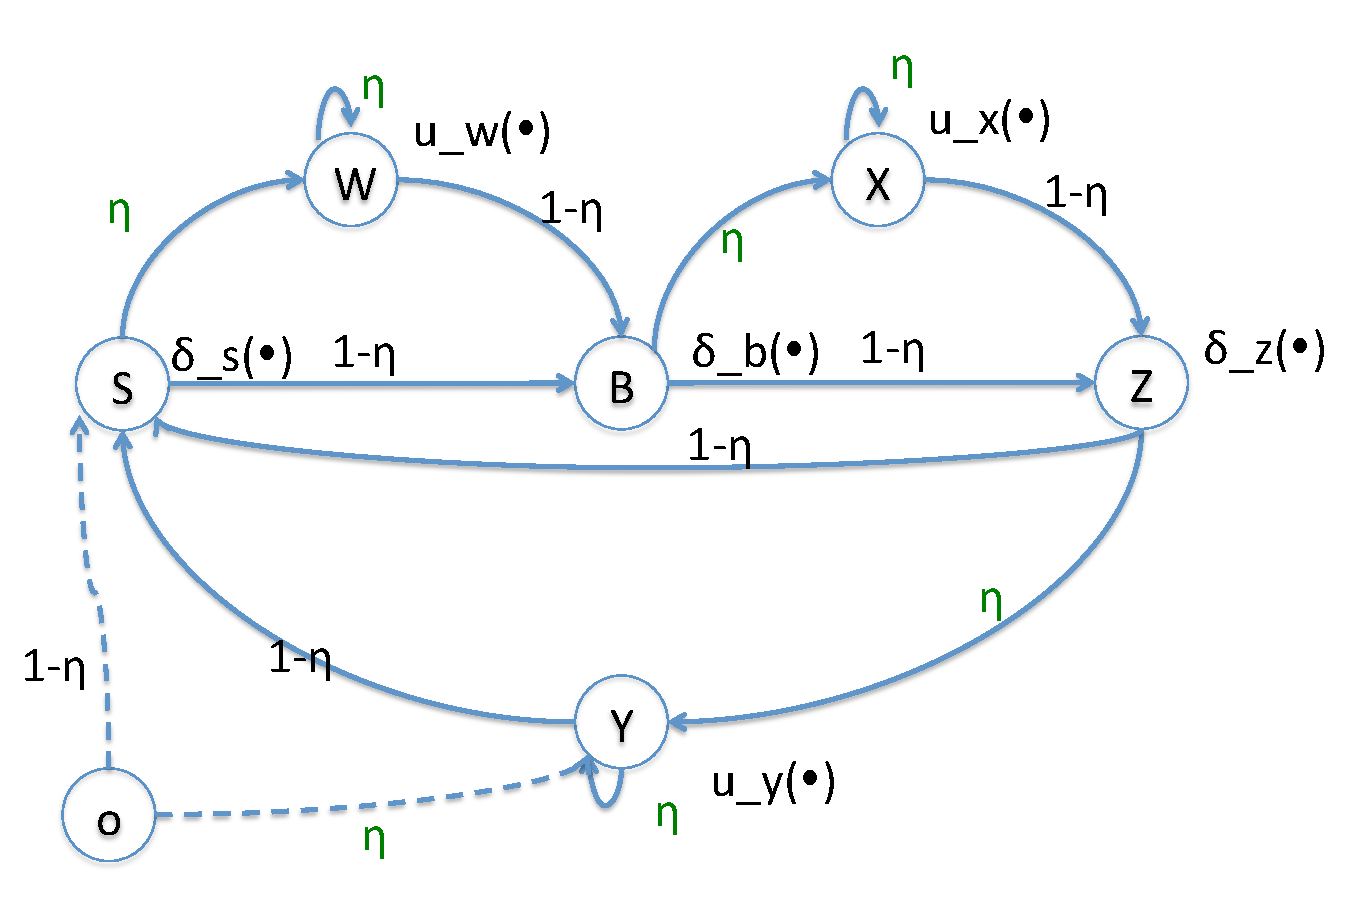
\includegraphics[width=0.5\textwidth]{adlfigs/egh.pdf}
\caption{States Transition of Episode Generating HMM (EGH).\label{fig_egh}}
\end{figure}


Theorem \ref{theorem1} from \cite{laxman2008stream} is crucial.  
The theorems in \cite{laxman2008stream}
prove that the more frequent an episode is inside a sequence, 
the greater the likelihood of the state sequence including this episode. 
The proof for this theorem is explained in detail in \cite{laxman2008stream}. 


\newtheorem{mydef}{THEOREM}
\begin{mydef}
\label{theorem1}~\cite{laxman2008stream} 
Let $D_Z={X_1,..., X_K}$ is the given sequence data,  $\varepsilon$ is the symbol set, 
and the size of these symbols is $M$. 
Given two frequent N-node episodes $\alpha$ and $\beta$ with frequency $f_{\alpha}$ 
and $f_{\beta}$. Their corresponding EGH is $\Lambda_{\alpha}$ and $\Lambda_{\beta}$. 
The most likely state sequence for episode $\alpha$ and $\beta$ are
$q_{\alpha}^*$ and $q_{\beta}^*$. 
The noise parameters of these two EGH are 
$\eta_{\alpha}$ and $\eta_{\beta}$. 
Assume both of these noise parameters are less than $\frac{M}{M+1}$, 
we have 
(1) if $f_{\alpha} > f_{\beta}$, then $P(D_Z, q_{\alpha}^*| \Lambda) > P(D_Z, q_{\beta}^*| \Lambda)  $
(2) if $P(D_Z, q_{\alpha}^*| \Lambda) > P(D_Z, q_{\beta}^*| \Lambda)  $, $f_{\alpha} > f_{\beta}$
\end{mydef}

\textbf{Mixture Model}
The mixture EGH model is fully discussed in previous work \cite{laxman2008stream}.
This model 
gives different weights to each EGH
to predict a target event. 
We can assume we obtain whether an episode occurs on a certain day. 
Let $D_Z=\{X_1,..., X_K\}$ denote the $K$ days data set. 
$F=\{\alpha_1, ... \alpha_J\}$ denote the frequent episodes in the dataset $D_Z$. 
An EGH $\Lambda_{\alpha_j}$ 
is associated with frequent episode $\alpha_j$.
$\Lambda_Z$ denotes a mixture EGH model. 
The likelihood of $D_Z$ under the mixture model is written as Equation (\ref{eq_mixture}).
\begin{eqnarray}
\label{eq_mixture}
Pr(\Lambda|Z) &=& \prod_{i=1}^K P[X_i|\Lambda_Z] \\
			&=& \prod_{i=1}^K ( \sum_{j=1}^J \theta_j P[X_i| \Lambda_{\alpha_j}])
\end{eqnarray}
where $\theta_j$ is the mixture coefficient of $\Lambda_{\alpha_j}$ and it subjects to 
$\sum_{j=0}^J \theta_j=1$ 

The parts inside Equation (\ref{eq_mixture}) are additive; 
the coefficients $\theta$ are computed by EM algorithm. 
%The detailed description is algorithm %%%\ref{alg3} 
%in the appendix section.
%% algorithm 03
\renewcommand{\algorithmicrequire}{\textbf{Input:}}
\renewcommand{\algorithmicensure}{\textbf{Output:}}

\begin{algorithm}
\caption{EM Algorithm for mixture EGH}
\label{alg3}
\begin{algorithmic} [1]
\REQUIRE day episode matrix, 
each element $e_{ij}$ records for each day whether an episode $j$ happens in day $i$;
frequent episodes $F=\{\alpha_1, ..., \alpha_J\}$;
symbol set $\varepsilon$;
threshold $\gamma$

\ENSURE the parameters for mixture EGH $\Lambda_Z=\{  (\Lambda_{\alpha_j}, \theta_j ) , j=1,...,J \}$


\STATE calculate the number of episodes J, and number of days K
\STATE calculate all $\eta$s' threshold value $mThreshold= \frac{M}{M+1}$

\COMMENT{initialize all the thetas to be $\frac{1}{J}$}
\COMMENT{calculate the total frequency for each episode over training time series}
\COMMENT{ calculate the $eta$ value}
\FOR{$0 \leq j \leq J$}
\STATE $\theta[j]= 1/J$
\STATE $episodeFreq[j] = \sum_i^K e_{ij}$
\ENDFOR

\STATE select those frequent episodes starting with 'S' and ending with 'Z' and separate these 
episodes by workday or holiday

\COMMENT {calculate $eta$ for each episode} 
\FOR{$0 \leq j \leq J$}
\STATE $\eta[j]= 1-episodeLen[j]*episodeLen/T$
\ENDFOR

\COMMENT{likelihood prediction of each episode $j$ in the $k$th day}

\FOR{$0 \leq i \leq K$}
\FOR{$0 \leq j \leq J$}
\STATE $likelihood_{ij} = \frac{1-\eta[j]}{\eta[j]/M} ^ {episodeLen[j]*e_{ij}}$
\ENDFOR
\ENDFOR

\COMMENT{calculate the obj value based on J, K, $likelihood_{ij}$ and $\theta$}
\WHILE{$newObj- obj > \gamma$}
\STATE $\theta_{new}=[]$
\FOR{$0 \le l \le J$}
\STATE $temp=0$
\FOR{$0 \le j \le K$}
%\COMMENT{calcuate the new likelihood with Bayes rules}
\STATE $temp = temp+ \frac{\theta_l*likelihood_{il}}{ \sum_0^J { \theta_j*likelihood_{ij}}}$

\ENDFOR
\STATE $\theta_{new}[l] = temp/K $
\ENDFOR

\STATE calculate the newObj
\IF{$newObj-obj > \gamma$}
\STATE $obj=newObj$
\STATE $\theta_{new} = \theta$
\ENDIF

\ENDWHILE

\STATE Output $\Lambda_Z=\{  (\Lambda_{\alpha_j}, \theta_j ) , j=1,...,J \}$

\end{algorithmic}
\end{algorithm}
During the initialization %line 1-10
part of the EM algorithm, 
the episode frequency over the times series T over $K$ days is calculated. 
Specific frequent episodes ended with target event 'Z' are selected. 
Optionally, 
we could add special constraints on episodes, starting with 
certain event type 'S'. 
%calculated in lines 11-16. 
% not sure this paragraph to be added or not
In the expectation step, 
one key part is the likelihood value of each episode $\alpha_j$ in time series $X_i$.
The likelihood value is computed as Equation (\ref{eq_likelihood});
Then Bayes rules is applied to compute the new coefficient $\theta_{new}$. 
\begin{equation}
\label{eq_likelihood}
Pr(X_i| \Lambda_{\alpha_j}) = (\frac{\eta_{\alpha_j}}{M})^{|X_i|} (\frac{1-\eta_{\alpha_j}}{\eta_{\alpha_j}/M})^{|\alpha_j|f_{\alpha_j}(X_i)}
\end{equation}
In the maximization step, 
we update the objective value based on Equation (\ref{eq_mixture}) until it converges, i.e., 
until the difference of two consecutive objective values 
is smaller than a threshold.%$\gamma$.


\subsubsection{Predict When the Target Event Occurs}
Target event prediction is studied in~\cite{laxman2008stream},  
but only insofar as it predicts whether a target event will occur, 
rather than when the target event will happen. 
Our occupancy prediction algorithm enriches the previous 
event prediction algorithm by breaking into three sub-problems; whether the target event un-occupancy $Z$ will appear, when the target event $Z$ starts, and when the target event $Z$ ends. 

Since the solution to the first sub-problem is similar to 
previous work, 
this sub-section emphasizes on the last two sub-problems. 
After obtaining the result of the first sub-problems, 
we assume we already know that the target event $Z$ will surely happen, 
and so we need to predict when the person leaves or comes back. 
The leaving time corresponds to the start time of dwelling event $Z.start$ and 
the returning time refers to the end time of dwelling event $Z.end$. 
%This prediction algorithm is described in algorithm \ref{alg22}. 

After running episode mining and mixing the EGH model, 
we have obtained all the frequent episodes $F=\langle \alpha_1,..., \alpha_J \rangle$, 
the corresponding EGH $\Lambda_{\alpha_j}, j=1...J$ with noise parameter $\eta_j$, 
and the mixture models $\Lambda_Z$ with coefficients $\theta_j$.
We use the coefficient of these mixture models to predict the leave time and return time of 
target event $Z$. 
 Each day is cut into three phases: 1) Before a person gets up; 
2) After the person gets up but before the person goes out;
and 3) After the person goes out but before they come back. 
\begin{enumerate}
\item
Usually before a person gets up, there is only one frequent episode named 'SZ'. 
The start time and end time of $Z$ depends on 'S'. 
Therefore $Z.start$ and $Z.end$  are calculated by the probability density function of 
going out and coming back time in the past days. 
\item
After the person gets up, if he/she has a lot of activities at home, 
there are several frequent episodes that are mined before the person leaves home. 
If there are several frequent episodes ending with $Z$,  
the leave time and return time of each episode is checked to determine
whether they are in a range of probability density function (PDF) value in the past. 
If yes, the mean value of these episodes are recorded. 
Since each episode generates an EGH, 
the mixture EGH model computes a weight for each EGH as coefficients. 
The leave time $Z.start$ and back time $Z.back$ are 
the weighted mean leave time and back time of these frequent episodes. 
\item
After a person leaves home, 
we already know when the person leaves home $Z.start$. 
If the person has come back, 
nothing needs to be predicted. 
If the person has not come back,  
the return time $Z.end$ is the weighted 
 historical return time of mined 
frequent episodes, 
viz. the probability density function of backing time based on the 
time-constraint going out time.
\end{enumerate}


 






%\section{Disaggregation Results}
\subsection{Evaluation for Disaggregation}
%The evaluation tools has been discussed in prior work \cite{liang2010load}.
%
%To evaluate whether each devices is disaggregated or not,
%we need to evaluate two parts, one is how much energy
%is evaluated compared to the ground truth. Another is
%among those disaggregated energy, how much percentage
%are disaggregated right.
%
I use precision, recall and F-measure in our evaluation. The standard
definitions of these metrics are:
%\begin{equation}
$\textrm{precision}=\frac{TP}{TP+FP}$, 
%\end{equation}
%\begin{equation}
$\textrm{recall}=\frac{TP}{TP+FN}$,
%\end{equation}
%\begin{equation}
$\textrm{F-measure}=\frac{1}{\frac{1}{\textrm{precision}}+\frac{1}{\textrm{recall}}}$
%\end{equation}

We need to define the notions of true/false positives
and negatives in the context of disaggregation.

Let us suppose there is a ground truth time series $x$ with length T, 
and denote the corresponding disaggregated time series by $\hat{x}$.
For any time $t \in (0, T)$, there are two values: the
ground truth value of device $m$ is $x_t^{(m)}$ and the disaggregated value
$\hat{x}_t^{(m)}$. We define a parameter $\rho$ for the range of
true values $x_t^{(m)}$, and another parameter $\theta$
as the noise.
For any given measurement, 
there are four total power values %or water usage values 
of device $m$ at
each point: true positive $TP^{(m)}$,  false negative $FN^{(m)}$,
true negative $TN^{(m)}$, and false positive $FP^{(m)}$.

\noindent
1. When $x_t^{(m)} > \theta$ and  $\hat{x}_t^{(m)}> \theta  $,
at this point the disaggregation is a true positive.
There are three situations in turn:

\noindent
1.1. When $  x_t^{(m)} \times (1-\rho) <  \hat{x}_t^{(m)} <  x_t^{(m)} \times (1+\rho)  $, then
\begin{eqnarray*}
 TP^{(m)} &=& \hat{x}_t^{(m)} \\
 FN^{(m)}&=&FP^{(m)} = TN^{(m)}=0
\end{eqnarray*}

\noindent
1.2. When $ \hat{x}_t^{(m)} < x_t^{(m)} \times (1-\rho)$ , then only
the disaggregated power %or water usage 
is considered as true positive and
the power %or water 
usage that is not disaggregated is regarded as a false negative:
\begin{eqnarray*}
TP^{(m)}&=&\hat{x}_t^{(m)} \\
FN^{(m)}&=&x_t^{(m)} - \hat{x}_t^{(m)} \\
FP^{(m)}&=&TN^{(m)}=0
\end{eqnarray*}
1.3 When $ \hat{x}_t^{(m)}>  x_t^{(m)} \times (1+\rho) $, then
the disaggregated power %or water 
usage is a true positive, and those values
which are greater than the truth values are treated as false positive.
\begin{eqnarray*}
TP^{(m)}&=&\hat{x}_t^{(m)} \\
FP^{(m)}&=&\hat{x}_t^{(m)} - x_t^{(m)} \\
FN^{(m)}&=&TN^{(m)}=0
\end{eqnarray*}
2. When $x_t^{(m)} > \theta$ and  $\hat{x}_t^{(m)}< \theta  $,
at this point the disaggregation is a false positive.  Then,
\begin{eqnarray*}
FP^{(m)}&=&x_t^{(m)} \\
TP^{(m)}&=&FN^{(m)} =TN^{(m)}=0
\end{eqnarray*}
3. When $x_t^{(m)} < \theta$ and  $\hat{x}_t^{(m)} > \theta  $,
at this point the disaggregation is a false negative. Then,
\begin{eqnarray*}
FN^{(m)}&=&x_t^{(m)} \\
TP^{(m)}&=&FP^{(m)} = TN^{(m)}=0
\end{eqnarray*}
4. When $x_t^{(m)} < \theta$ and  $\hat{x}_t^{(m)} < \theta  $,
at this point the disaggregation is a true negative.  Then,
\begin{eqnarray*}
TP^{(m)}&=&FN^{(m)} = FP^{(m)} = TN^{(m)}=0
\end{eqnarray*}
%In practice, we use different
%$\rho$ and $\theta$ values depending on the
%dataset. For instance, considering the datasets described below,

In our experimental dataset, we set
$\theta=100$ and $\rho=0.2$. 
Although the maximal power consumption of all these devices is 11000W, 
we can still set $\theta < 11000 * 0.1$ because we apply multivariate piecewise motif mining recursively, 
so the devices which consume a large amount of power are deleted in the first few rounds. 
Therefore the power noise which is caused by the high-power electronic devices 
is greatly decreased. 

\subsection{Disaggregation Experiments}
We run experiments on the dataset Study10 from the University of Virginia on electricity disaggregation. 
This dataset collects data from 02/10/2014 to 02/21/2014 in a residential building. 
%the following paragraph is from UVa
Two individuals were asked to live in an instrumented home for around two weeks. 
To ensure the data consisted of the personal usage patterns of the participants, 
they were encouraged to live in and use the home as they normally would use their own. 
%The study had institutional review board (IRB) approval and each participant received a \$100 incentive. 
An eMonitor \cite{eMonitor} sensor was used to collect both mains data for testing and circuit-level information for ground truth. 
Additional data, such as the opening of appliance doors and the flicking of light switches, 
was collected to provide sub-circuit level ground truth information for events such as lights.
Both the two-phase aggregated data and each device's data are collected at intervals of 2-3 seconds.
In total, 25 devices were connected to two phases at the entry of the house. 
Five of these devices are seldomly operated; less than five times. 
Fourteen devices consume power less than 100W, and the majority of them are lights. 
The largest power consumption of these devices is 11000W by indoor heating. 
The noise caused by the heating device is large; greater than 100W. 
Therefore we focus on disaggregating the six major electronic devices 
with power levels greater than 100W. 
 
% the datasets from University of Virginia on both water and electricity disaggregation. 
%There are totally six data sets. The statistic of these six data set is listed in Table \ref{table_datasets}. 
%The recording interval of these datasets is 2 or 3 seconds. 
%A sensor is instrumented on each device to trace its ground truth operations. 
%\input{tab/datasets}

\subsubsection{Electricity Disaggregation}
We assume that we know the power levels of each device. 
If the power levels of each device are unknown, 
we can use the sum of two-phase aggregated data and the on/off events of the 
ground truth to extract them. 
%In order to extract the power level of each device, 
We set a window size $w=30s$ ahead and behind of the ground truth events to match 
the aggregated data.
If there is only one power change in the aggregated data during these 60 seconds, 
this power level change must come from an on/off event of an electrical device. 
Usually, it takes around 2-5 seconds for an electrical device to reach
a steady power level. 
The on and off events reflect different durations for a device to 
reach a steady state. 
Therefore, we measure the minimal duration of the on event and off event 
of each device. 
\input{multidisaggtab/study10results}
After we go over all the aggregated data and ground truth on/off events, 
we run a Gaussian mixture model to model the positive power changes and negative power changes
independently. The means and standard deviations correspond to  the on/off event of each device. 
The power levels, standard deviation, and on/off duration of each device of dataset study10 are listed in Table \ref{table_study10results}.

%By analyzing each device, we notice that sometimes the power levels and 
%on/off duration are insufficient to identify the electric devices. 
%For instance, when the device heatingIndoor starts alone, 
%it takes $2-5$ seconds to go to a steady state as shown in Figure \ref{fig_heatingDevices} (a).
%But when the combined device of heatingIndoor and heatingOutdoor 
%starts, the starting duration takes around $4-18$ seconds. 
%In Figure \ref{fig_patterns} (b), after this combined device 
%starts for15 seconds, the power levels changes 
%for 9 times then to a relatively stable state. 
%During this period of 15 seconds, the power changes very rapidly. 
%If we accumulate these power levels together, 
%it's not a fix number. Therefore, for this kind of device, 
%we can only compare the shape of the startup to decide the on events 
%from the aggregated data. 

We apply recursive multivariate piecewise motif mining to dataset Study10 
and compute the precision, recall and F-measure. 
Devices which draw power from both phases are separated first. 
They are heatingIndoor, waterheater and dryer.
\input{multidisaggfig/heatingIndoorResults}
Figure \ref{fig_heatingIndoorResults} (a) gives an example of 
an on event in the two-phase Mains1 and Mains2. 
Mains1.diff denotes the diffs data from Mains1 and Mains2.diff represents 
the diffs data from Mains2. 
Mains1.2.diff shows as blue when Mains1 and Mains2 share the similar power changes. 
We can see that 
the power consumption of a specific device jumps twice in two phases simultaneously.
The first time, both phases jump 2572W. After nine seconds, 
the power of both phases increases  2520W. 
The sum of these four changes is 10184W. 
Compared with the power levels of all devices, 
we speculate that these power changes are caused 
by the device heatingIndoor. 
%By applying multivariate piecewise motif mining, 
%we match the power consumption with $11000W$ and 
%categorize this on event into heating indoor. 
Figure \ref{fig_heatingIndoorResults} (b) shares the same snippet of time series as Figure \ref{fig_heatingIndoorResults} (a). 
The red line indicates that the on event of heatingIndoor is recognized.    
\input{multidisaggfig/dryerResults}
Similarly, the off event plunges twice in two seconds -2877W and -1759W in both phases, as shown in Figure \ref{fig_heatingIndoorResults} (c).
The sum of this off event is -9272W. 
After matching the power levels, we categorize it as the off event of heatingIndoor as indicated in Figure \ref{fig_heatingIndoorResults} (d). 

The dryer has the same power level as the waterheater at around 4800W. 
If we disaggregate these two devices from the sum of the two phases, 
it's difficult to distinguish them,  
but with multivariate piecewise motif mining, these two devices 
can be distinguished. 

%Figure \ref{fig_dryerResults} (a) and (b) shows the on event of dryer from sum of phase 1 and phase 2, 
%and these two phases separately. 
Figure \ref{fig_dryerResults} (a) and (b) are the diff data of the dryer and waterheater from the two-phase circuit. 
We can see that the waterheater draws power from Phase 1 and Phase 2 at the same time,  
but the dryer shows a different pattern. It draws power from Phase 1 at a lower power of 1093W, then jumps to 1830W; 
at the same time, it draws power from Phase 2 at the high level of 1946W immediately. 
We encode the power usage as shown in Figure \ref{fig_eventEncoding}, then apply motif mining to disaggregate them. 
 
After deleting the power consumption from both aggregated phases, 
we apply piecewise motif mining again to a single phase. 
We then discover the humidifier from Phase 1 
and the microwave from Phase 2. 
%Note that the power consumption of humidifier and microwave overlaps sometimes, 
%which makes it hard to separate them. 
%But they draw power from different phases separately. 
%Multivariate motif mining can separate them. 
When we only disaggregate the sum of Phase 1 and Phase 2, 
the precision recall result of the microwave and humidifier is not very accurate 
because sometimes their power consumptions are similar. 
However, using multivariate motif mining, we can separate them very clearly 
with good precision and recall. 
The precision and recall results for the data set Study10 are listed in Table \ref{table_study10results}.

Recursive multivariate motif mining is capable of disaggregating continuous variable loads. 
%\input{multidisaggfig/heatingOutdoorResults}
Figure \ref{fig_dryerResults} (c) shows the diff data of heatingOutdoor from the two phases. 
During this on event, its power levels change nine times, then continue at a relatively stable state.
%Figure \ref{fig_heatingOutdoorResults} (a) illustrates the startup of heatingOutdoor.
%as shown in Figure \ref{fig_heatingOutdoorResults} (b) and (c). 
By applying piecewise motif mining, 
we can successfully identify this as the heatingOutdoor device 
after matching its power level. 
%The disaggregated result is displayed in Figure \ref{fig_dryerResults} (d).
%Note that this continuous variable load startup snippet can be discovered by dynamic time warping 
%subsequence search as well if this device is on without the intervene of other devices.
If another device  $D$ which draws from Phase 1 or Phase 2 is turned on or off during this period, 
multivariate piece-wise motif mining can still identify this heatingOutdoor device. 
This is because $D$ only uses one phase's power; 
hence its power change is not counted in our piecewise event. 

\iffalse
\subsubsection{Water Disaggregation and Constraints}
Water usage displays different characteristics. 
The total water consumption is zero most of the time.
Whenever a water use end is operated, water is consumed intensively for a period of time. 
Then it will stay off for a much longer time. 
We observe that the operations of water use ends reflect a series of user behaviors. 
For instance, a person may use the toilet in the bathroom first, 
then wash hands in the sink and finally take a shower afterwards. 
%This series of events highly affect electricity usage as well. 
%When the person enters into the bathroom, the light in the bathroom is turned on. 
%After using the bathroom, the person leaves and turns the light off. 
%Moreover, we observe that the usage of toilet is usually accompanied by
%sink usage afterwards. 

%In this subsection, we apply the semi-supervised multivariate piecewise motif mining 
%to water data. 
Similar to electricity disaggregation, we use a period of aggregated water usage 
data to extract features  
and obtain the water flow rate level of each water use end.
Table \ref{table_resultStudy10Water} lists the water consumption rate for each device. 
For instance, taking a shower uses hot water at a flow rate between 0.1822 liter/min and 0.1986 liter/min. 
Let $\frac{\alpha}{10000}$ denotes this range of water flow rate.
The total hot and cold water consumption by  shower is 0.1904 liter/min. 
Therefore, the cold water flow rate caused by shower is $0.1904-\frac{\alpha}{10000}$ liter/min. 
Turning on the water for the shower takes around two seconds. 
%The disaggregation results are shown in Table \ref{table_resultStudy10Water}.
%\input{multidisaggtab/study10waterresults}
\begin{table}[h]
\renewcommand{\arraystretch}{1.3}
%\caption{Water Flow Rate Levels of Water End Uses.}
%\label{table_resultStudy10Water}
\tbl{Water Flow Rate Levels of Water End Uses and Disaggregation Results.\label{table_resultStudy10Water}}{
\centering
\small
\setlength\tabcolsep{2pt}
\begin{tabular}{|c|c|c|c|c|c|c|}
\hline
\multirow{2}{*}{Device} & \multirow{2}{*}{Hot water} & \multirow{2}{*}{Cold water} & \multirow{2}{*}{Duration}  \\
           &  (liter/min*10000) & (l/min*10000)  & (second)\\
\hline
\hline
Shower & $\alpha \in (1822, 1986)$ & $1904-\alpha$  & on: 2\\
\hline
Washing Machine & $\alpha \in (1988, 2276)$  & $2132-\alpha$ & on: 5\\
\hline
DownToilet & 0 & (1270, 1400) & whole: 50\\
\hline
UpToilet & 0 & (1480, 1700) & whole: 50\\
%\hline
%KitchenSink &  $ \alpha \in (0, 57) $ & 57- $\alpha$ & 2& & & \\
%\hline
%UpSink & 34 & 160 & 2& & & \\
%\hline
%DownSink & 57  & 80 & 2& & & \\
%\hline
%Dish Washer & 34 & -11 & 2& & & \\
\hline
\end{tabular}
}
\end{table}

After these calculations, we apply a multivariate piecewise motif mining approach to 
water disaggregation. 
For the shower and washing machine, 
the total flow rate of hot and cold water is high,  nearly 0.2 liter/minute. 
Therefore by only searching the 
total hot and cold water flow rate, we can identify these two devices. 
The event of shower usage usually lasts for more than one minute, 
but the washing machine uses water for less than one minute, 
repeating six to nine times. 
Both the shower and washing machine use 
hot water and cold water. 
However, the washing machine uses hot water for only the 
first one or two times. For the rest of its cycle, 
only cold water is used. 
Whenever the washing machines starts, 
the power consumption starts as well. 

%\input{multidisaggfig/waterDisaggResults}
%Figure \ref{fig_waterDisaggResults} (a) and (b) display the water usage of shower and washing machine. 
Applying piecewise motif mining to the water usage lets us disaggregate the
shower and washing machine. %as in Figure \ref{fig_waterDisaggResults} (a) and (b).
The precision, recall and F-measure for the shower disaggregation are 
0.999, 0.972, and 0.986,  
and the precision, recall and F-measure for the washing machine disaggregation are 
0.997, 0.969, and 0.983. 
However, with a variable water flow rate, 
piecewise motif mining has limitations in handling water use ends such as the toilet.
Therefore we use the dynamic time warping subsequence~\cite{rakthanmanon2012searching} search as a complementary to discover these water use ends.  
For the two toilets, we apply dynamic time warping to match the time series.
The water usage results of one toilet, UpToilet, is shown in Figure \ref{fig_dryerResults} (d). 

%There are totally three sinks in the house, namely up sink, down sink and kitchen sink. 
%People may use sinks with only hot water or cold water, or both hot and cold water. 
%The water usage may be large or small. 
%In this case, it is hard to distinguish these three sinks. 
%However, by observing the water usage of up sink and down sink. 
%We find that there's correlation between the down sink and the down toilet, 
%up sink and up toilet. 
%Figure \ref{fig_ToiletSinkCorrelation} (a) and (b) show that the toilet and sink start almost at the same time, 
%or end at the same time. 
We can see that multivariate piecewise motif mining is capable of 
disaggregating water use ends which have sharp on/off water flow rates. 
However, it has limitations in dealing with water use ends with irregular water use patterns, 
such as toilets and sinks. 
Since the water usage of toilets is relatively fixed if used alone, 
some toilet water usages can be disaggregated by using the dynamic time warping subsequence search 
which was researched in \cite{nguyen2013development}. 
\fi

\section{Experiment Results of Occupancy Prediction}
We have conducted experiments on three datasets, where each dataset is obtained by monitoring 24-hour activities of two adults in a house via RFID. 
All these activities occur in twelve rooms; the basement, bathroom, bedroom, dining room, hallway, kitchen, living room, mudroom, nursery, outside-front, outside-back, and upstairs. 
The dataset comprises events in the form of timestamped room occupancy data points. For instance, an event can correspond to person 1 being in the kitchen at 7:00 am. The summary of these three datasets is shown in Table~\ref{tab_dataset}. 
\begin{table}[h]
\centering
\caption {Datasets summary.} \label{tab_dataset}
%\tbl{Datasets summary.\label{tab_dataset}}{
%\vspace{0.2cm}
\begin{tabular} {|c|c|c|c|}
\hline
Dataset & Number of entries & Period(day) & Start date\\
\hline
study10  & 6596 & 12 & 02/10/2014\\
\hline
study11  & 1696 & 10 & 01/29/2014\\
\hline
study14 & 3453 & 13 & 12/09/2013\\
\hline
\end{tabular}
%}
%\end{center}
%\end {table}
%\end{minipage}%
\end{table}
%Study10 spans 12 days from 02/10/2014 to 02/21/2014 and Study11 spans 10 days from 01/29/2014 to 02/07/2014, and Study14 spans 13 days from 12/09/2013 to 12/21/2013.
We define \textit{unoccupancy} of a person as one of these conditions: the person leaves the {\em outside-front} or {\em outside-back} for more than 30 minutes; the person stays in the living room or dining room for more than 9 hours without any other activities; or the gap between any two events is more than 30 minutes. 
Since our research goal is to automate the turning on and off of the HVAC system at least 30 minutes before occupancy, the first and third constraints are in place. We are only interested in events where the {\em unocupancy} period is for an extended duration ($>$ 30 minutes). The second constraint comes from our observation that if a person stays in one room for more than 9 hours without moving to other rooms, 
this usually means that the person has gone out but left the RFID equipment at home. 
Furthermore, we delete events with a duration less than 
2 minutes since these correspond to the individual walking back and forth across rooms and generally do not contribute to meaningful episodes. We conduct four types of experiments to compare four approaches; 
kNN, mixture EGH, PDF, and support vector regression (SVR). 
For each dataset, we use $2/3$ of the data for training and the remaining $1/3$ of the data as a test. 
Following the approach in~\cite{scott2011preheat},
we organize one day's data into 96 15-minute chunks. 
For the test data, we assume that we only know some of the 15-minute chunks. Our target is to predict the occupancy in the rest of the day, or 30 minutes ahead. 

\subsection{Occupancy Prediction of Individuals}
%We apply three approaches, kNN, PDF based and mixture EGH time prediction model. 
%Similar to \cite{scott2011preheat},
%we organize one day's date into 96 15-minutes intervals with mixture EGH model. 
%Then we split the test date into three phases: 
%(1) before getting up, (2) after getting up and before going out, 
%(3) after going out and before coming back. 
%Thus our problem becomes to predict when the person going out 
%and when the person comes back. 
%Corresponding to these four phases, we adopt three different approaches. 
%For stage (1), the probability density function of going out and combing back event is calculated. 
%For stage (2), a duration-constraint episode mining and episode generative HMM is applied. 
%For stage (3), the probability density function of backing time based on 
%the time-constrains going out time is computed. 

%The results are shown in Figure~\ref{fig_study10} and Table~\ref{tab_individualResults}
%Figure~\ref{fig_study11}, and Figure~\ref{fig_study14}. 
%Each of these figures 

\begin{table*}[t]
%\vspace{0.2cm}
\hfill
%\begin{minipage}[t]{1.0\linewidth}%

\caption{Precision Recall F-measure Comparison of Individual and Whole House Occupancy Prediction in Study 14.}
\label{tab_individualResults}
%\tbl{Precision Recall F-measure Comparison of Individual and Whole House Occupancy Prediction in Study 14.\label{tab_individualResults}}{
%\begin{center}
%\makebox[\textwidth]{
\centering
\small
\setlength\tabcolsep{2pt}
\begin{tabular} {|l|l|l|l|l|l|l|l|l|l|l|l|l|l|l|l|}
\hline
\multirow{2}{*}{Dataset}&\multirow{2}{*}{Date}&\multirow{2}{*}{Person} & \multicolumn{3}{|c|}{EGH}&\multicolumn{3}{|c|}{kNN} &\multicolumn{3}{|c|}{SVM}   \\
\cline{4-12}
&&& precision & recall &fmeasure &precision & recall & fmeasure &precision & recall & fmeasure \\
\hline
\multirow{3}{*}{study10}  & 02/17/2014 & person2& \textbf{1.00} & \textbf{1.00}&\textbf{1.00} & 0.99 & 0.98 & 0.98 &0.71 &0.76 & 0.71\\
\cline{2-12}
& 02/19/2014 & person1& 0.98 & 0.99 &0.98&  \textbf{0.99} &  \textbf{0.99} &  \textbf{0.99} & 0.71 & 0.76 & 0.70 \\
\cline{2-12}
& 02/20/2014 & person2&  \textbf{0.93} &  \textbf{0.92} &  \textbf{0.92} & 0.92 & 0.91 & 0.90 & 0.72 & 0.77 & 0.72\\
\cline{2-12}
& 02/20/2014 & person1&  \textbf{0.95}& \textbf{0.94} & \textbf{0.94} & 0.94	& 0.93 & 0.93 & 0.71 & 0.77 & 0.72 \\
\cline{2-12}
& 02/20/2014 & \textbf{wholehouse}&  \textbf{0.92}& \textbf{0.92} & \textbf{0.91} & 0.91	& 0.89 & 0.91 & 0.79 & 0.74 & 0.74 \\
\hline
\hline
\multirow{3}{*}{study11}  & 02/04/2014 & person2& 0.93 & 0.93 & 0.92  & \textbf{0.95} & \textbf{0.95} & \textbf{0.95} & 0.71 & 0.77 &0.72\\
\cline{2-12}
& 02/04/2014 & person1& 0.93 & 0.93 & 0.92  & \textbf{0.95} & \textbf{0.95} & \textbf{0.95} & 0.70 & 0.77 & 0.71  \\
\cline{2-12}
& 02/05/2014 & person2&  \textbf{0.85} &  \textbf{0.92} &  \textbf{0.86} & 0.87 & 0.87 & 0.84 & 0.71 & 0.76 & 0.71 \\
\cline{2-12}
& 02/05/2014 & person1&  \textbf{0.84} &  \textbf{0.90} &  \textbf{0.84} & 0.79 & 0.90 & 0.80  & 0.70 & 0.77 & 0.71   \\
\cline{2-12}
& 02/04/2014 & \textbf{wholehouse}&  \textbf{0.918}& \textbf{0.924} & \textbf{0.913} & 0.916	& 0.921 & 0.911 & 0.77 & 0.69 & 0.71  \\
\cline{2-12}
& 02/05/2014 & \textbf{wholehouse}&  \textbf{0.90}& \textbf{0.84} & \textbf{0.84} & 0.88	& 0.81 & 0.81 & 0.74 & 0.70 & 0.70\\
\hline
\end{tabular}
%}
%\end{center}
%\end{minipage}%
%\hfill%
\end{table*}
The individual occupancy prediction results on datasets Study10 and Study11 are summarized in Table~\ref{tab_individualResults}. 
In Study10,  the mixture EGH performs better than kNN for the occupancy prediction for person2 on 02/17/2014. 
Furthermore, mixture EGH outperforms kNN for both persons on 02/20/2014. 
However, for person1 on 02/19/2014, kNN works a little bit better. 
When checking the original data on this test date, 
we find that the activities on this date are very similar to the historical activities in the training data.
%\textbf{When checking the original data, we find that the date on that day is similar to the historical data. - need to rephrase}
This observation leads us to the conclusion that when the test data is very highly similar to the historical data, 
the kNN approach sometimes performs a little better.  
In Study11, mixture EGH gets higher precision, recall and f-measure scores on 02/05/2014, but the opposite is true on 02/04/2014. 
We analyzed the original data to find the reason for the kNN's better performance, and found the date is an anomaly from the normal pattern, since both individuals went to sleep late that day (after 12:00am).
Before sleep, person1 even stayed in the kitchen for around two hours. 
The frequent episode $KZ$, which represents 'kitchen-unoccupied', 
usually occurs in the morning instead of around midnight. 
However, the mixture EGH model still assumes that the $KZ$ pattern 
happens during the morning; 
therefore the prediction results are not accurate. 
%\textbf{On the contrary, 
%kNN doesn't consider the 
%actual place inside the room. - need to rephrase}
Since kNN ignores this fine granular activity pattern at a house and only considers the occupancy status in the past most similar five days, its performance is better. 
Generally speaking, the mixture EGH helps predict when a person 
leaves home and the period of sleeping and its 
performance is competitive to the kNN approach. 
For all these experiments, the SVR approach performs the worst because 
of the limitations of this approach. 
SVR uses the latest several data points about the occupancy state as the 
training vector for the prediction of the next occupancy state. 
Here we set eight past data points as the predictor. 
Other features such as the time of day and day of week cannot be utilized fully. 

We also conduct experiments for individuals' {\em rest-of-day} occupancy prediction at different times. 
\begin{figure}[h]
\centering
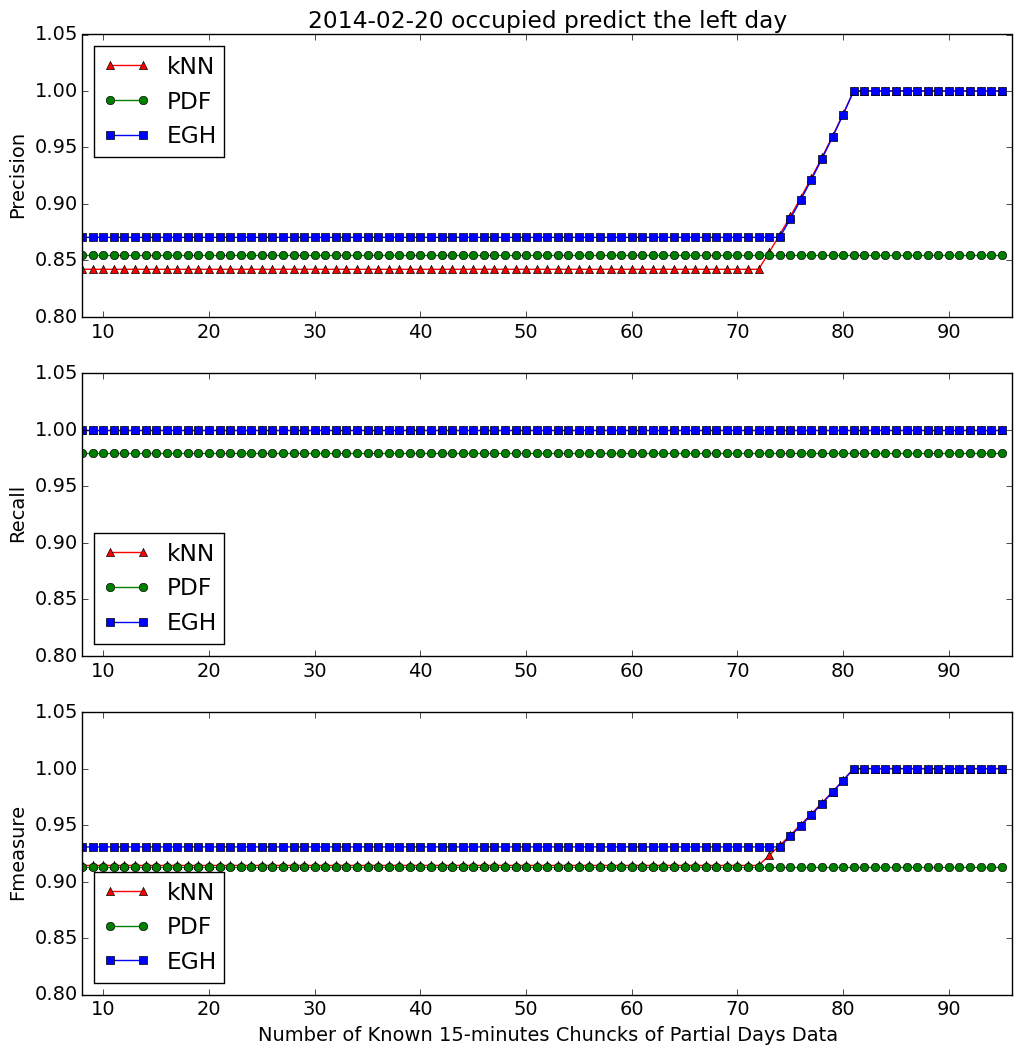
\includegraphics[width=0.7\textwidth]{adlfigs/study10person12014-02-20occupied.png}
\caption{Occupancy prediction precision, recall and f-measure comparison of three approaches 
of person1 on 02/20/2014 on Study10.}
\label{fig_study10}
\end{figure}
Figure~\ref{fig_study10} illustrates a person's occupancy prediction result in Study10.
There are three sub-figures. 
Each sub-figure describes the 
precision, recall, and f-measure 
of $person1$ on 02/20/2014. 
The blue line represents the mixture EGH model,
the green line represents the PDF model,
and the red line denotes the kNN model. 
The x-axis is the number of known 15-minute chunks of the test day. 
For instance, at $x=20$, 
we already know $20*15$ minutes' data 
and need to predict whether the home is occupied during the remaining $76$ chunks. 
The y-axis denotes the precision, recall and f-measure values 
in the three sub-figures from the top down. 
The first sub-figure shows that  
the mixEGH has the highest precision, recall and f-measure on test day 02/20/2014 
for occupancy prediction. The other two baseline approaches are comparable, except that kNN performs better than PDF 
when the person comes back home after slot 72. 
Looking into the original data, we find that person1 actually comes home later than usual 
in the training dataset. 
%In such case, mixture EGH performs best.  
%Figure \ref{fig_study10} (c) and (d) gives the occupancy and un-occupancy results 
%of person2 on 02/17/2014. 
%In such case, EGH mixture model performs best from the perspective of precision, recall and f-measure. 

\iffalse
Figure~\ref{fig_study14} (a) and (b) describe the case of person1 on 12/18/2013. 
Similar to Figure \ref{fig_study11} (a) and (b), 
mixture EGH model doesn't perform well before the person1 gets up 
and the reason keeps the same. 
The person1 slept late and some confused episodes are generated. 
Figure \ref{fig_study14} (c) and (d) describe the case of person1 on 12/19/2013. 
kNN performs better. MixtureEGH doesn't perform well because 12/19, 02/20 the person went out again after coming back and staying home for some time. However the training data don't include such case. 
\begin{figure}[h]
\centering
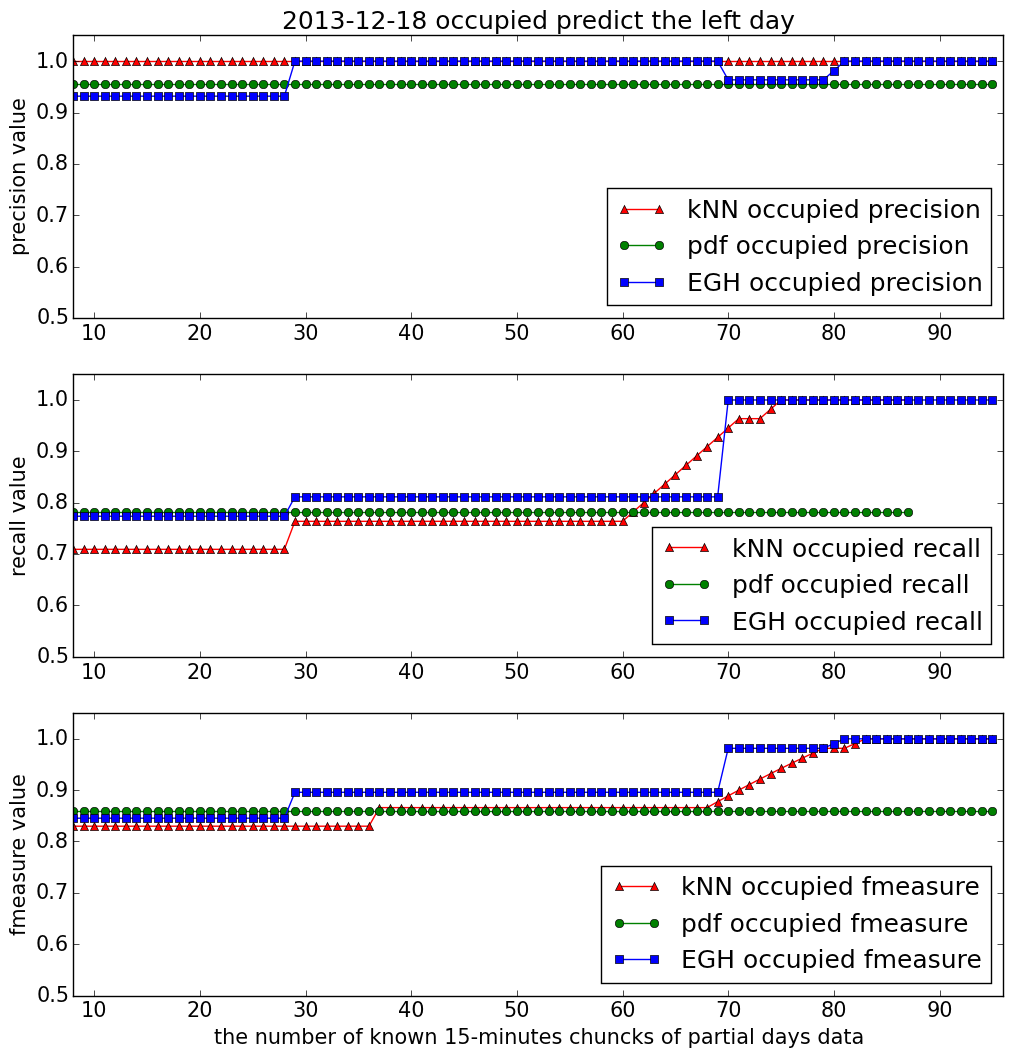
\includegraphics[width=0.5\textwidth]{adlfigs/study14person12013-12-18occupied.png} 
\caption{Study 14 Precision recall and f-measure comparison of three approaches.
person1 occupied 12/18/2014.}
\label{fig_study14}
\end{figure}
\fi


\subsection{Occupancy Prediction of Residential Buildings}
Based on individual prediction results, we deduce when a house is occupied
using logic OR operations on the prediction results of two persons. 
The whole house occupancy prediction results are listed in 
Table~\ref{tab_individualResults} and marked in bold. 
In Study10, the precision, recall, and fmeasure values of the whole house are 0.92, 0.92 and 0.91, respectively,  
which are higher than the values from the kNN approach of 0.91, 0.90 and 0.91, and of the SVR approach 0.79, 0.74 and 0.74. Similarly, the mixture EGH model outperforms kNN in Study11. 
Note that in Study 11 on 02/04/2015, 
EGH does not perform as well as kNN on individuals
but performs a little bit better than kNN, and much better than SVR in occupancy prediction of the whole house. 
The reason behind this is because the activities of the two people inside the home 
are not synchronized. The mixture EGH model can predict the 
occupancy for each person and grasp each person's activities more accurately. 
%When applying the logic OR operations on these two persons, 
%for whole-house occupancy prediction. 
\subsection{Limitations of Mixture EGH Model}
Although the temporal mixture EGH model performs well on the datasets Study10 and Study11, 
the same is not true for the dataset Study14. 
Table~\ref{tab_resultsLimitation} shows that, 
in Study14, 
the mixture EGH model works better for the individual and whole-house occupancy predictions on 12/18/2013 but not on 12/19/2013 or 12/20/2013. 
We check the activities of both individuals on these two days 
and find that both of them went out again 
after coming back and staying home for a while.
Since the episodes of going out after coming back home from work 
do not occur frequently, mixture EGH cannot detect this pattern. Thus the occupancy prediction probability of these events 
is completely missing. However kNN performs well because it leverages all the 
historical data; therefore, even if the abnormal event occurs once, 
this prediction approach incorporates it and obtains the average value. 
To relax the limitations of abnormal events, 
we propose a hybrid model for prediction;
when deploying this occupancy prediction in reality, 
for example for a prediction that is 30 minutes ahead, 
just 15 minutes before the prediction, if a person goes out again after coming back, 
the deployed system switches to the kNN approach rather than the mixture EGH model for prediction. In such cases, this hybrid model can always get the best prediction results. 

\begin{table*}[!t]
%\vspace{0.2cm}
\hfill
%\begin{minipage}[t]{1.0\linewidth}%

\caption{Precision Recall F-measure of Individual and Whole House Occupancy Prediction in Study 14.}
\label{tab_resultsLimitation}
%\tbl{Precision Recall F-measure of Individual and Whole House Occupancy Prediction in Study 14.\label{tab_resultsLimitation}}{
%\begin{center}
%\makebox[\textwidth]{
\centering
\small
\setlength\tabcolsep{2pt}
\begin{tabular} {|l|l|l|l|l|l|l|l|l|l|l|l|}
\hline
\multirow{2}{*}{Dataset}&\multirow{2}{*}{Date}&\multirow{2}{*}{Person} & \multicolumn{3}{|c|}{EGH}&\multicolumn{3}{|c|}{kNN} & \multicolumn{3}{|c|}{SVM} \\
\cline{4-12}
&&& precision & recall &fmeasure &precision & recall & fmeasure &precision & recall & fmeasure  \\
\hline
\multirow{3}{*}{study14}  & 12/18/2013 & person2&  \textbf{0.91} &  \textbf{0.91} &  \textbf{0.89} & 0.87 & 0.87 & 0.84 & 0.73 & 0.77 & 0.71\\
\cline{2-12}
& 12/18/2013 & person1&  \textbf{0.92} &  \textbf{0.92} &  \textbf{0.91} & 0.90 & 0.90 & 0.89 & 0.73 & 0.76 & 0.71 \\
\cline{2-12}
& 12/19/2014 & person2& 0.86 & 0.86 & 0.85  & \textbf{0.90} & \textbf{0.90} & \textbf{0.88} & 0.73 & 0.76 & 0.71\\
\cline{2-12}
& 12/19/2014 & person1& 0.85 & 0.84 & 0.84  & \textbf{0.86} & \textbf{0.86} & \textbf{0.85} & 0.73 & 0.76 & 0.71 \\
\cline{2-12}
& 12/20/2014 & person2& 0.92 & 0.94 & 0.92  & \textbf{0.98} & \textbf{0.97} & \textbf{0.97} & 0.75 & 0.79 & 0.75 \\
\cline{2-12}
& 12/20/2014 & person1& 0.90 & 0.91 & 0.90  & \textbf{0.95} & \textbf{0.95} & \textbf{0.95} & 0.75 & 0.79 & 0.75\\
\cline{2-12}
& 12/18/2013 & \textbf{wholehouse}&  \textbf{0.91}& \textbf{0.91} & \textbf{0.90} & 0.88	& 0.88 & 0.86 & 0.75 & 0.72 & 0.70 \\
\cline{2-12}
& 12/19/2013 & \textbf{wholehouse} & 0.841	& 0.845 & 0.838&  \textbf{0.848}& \textbf{0.853} & \textbf{0.842} & 0.79 & 0.74 & 0.74 \\
\cline{2-12}
& 12/20/2013 & \textbf{wholehouse} & 0.92	& 0.90 & 0.90&  \textbf{0.94}& \textbf{0.93} & \textbf{0.93} & 0.74 & 0.72 & 0.70 \\
\hline
\end{tabular}
%}
%\end{center}
%\end{minipage}%
%\hfill%
\end{table*}
\subsection{House Occupancy Prediction 30 Minutes Ahead with Hybrid Approach}
To preheat the house, we need to evaluate how much time in advance to automatically turn on/off HVAC, and the advance notice time estimation is given in~\cite{scott2011preheat}. 
Here we use prediction of 30 minutes ahead of time house occupancy. 
%because it is reasonable for preheating. 
We compare the receiver operating characteristic (ROC curve) of three approaches: mixture EGH model,  kNN, and a hybrid approach of the mixture EGH model and kNN. 
In this hybrid approach, 
we set mixture EGH results as the baseline, 
then replace the values of the mixture model by the values from kNN model 
in the following two situations: 
1) After a person comes back home; and 2) When the prediction probability of kNN is greater than 0.8. 
Figure~\ref{fig_rocresults_1}, ~\ref{fig_rocresults_2}, and~\ref{fig_rocresults_3} illustrate the ROC curve of the whole house occupancy prediction on 02/20/2014 of dataset Study10, 02/04/2014 of dataset Study 11 
and 12/20/2013 of dataset Study14, respectively.  
The red and green lines represents the kNN and mixture EGH models; 
the blue line denotes the hybrid approach. 
The ROC curves show that the hybrid approach always has the largest area, namely 
0.96, 0.92 and 0.92, 
which indicate that the hybrid approach always performs best. 
%\begin{figure}[h]
	\centering{
		\begin{tabular}{cccc}		
		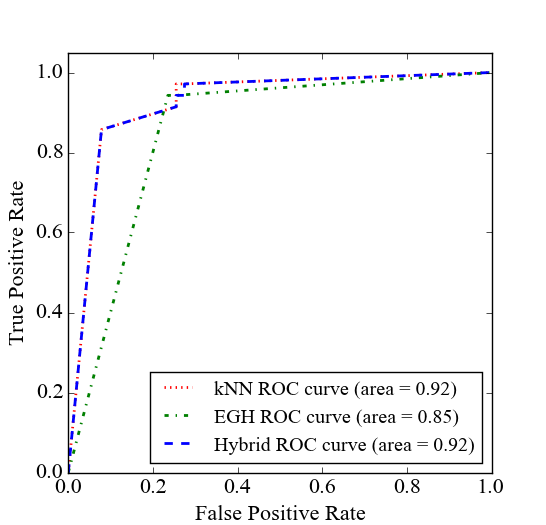
\includegraphics[width=0.5\textwidth]{adlfigs/study10ROC_02202014.png} &
		\tabular newline
		(a)\tabularnewline
		\end{tabular}
		}
	\caption{
	ROC curve of house occupancy prediction in Study10 (02/20/2014).}
	\label{fig_rocresults_1}
\end{figure}

\begin{figure}[h]
	\centering{
		\begin{tabular}{cccc}		
		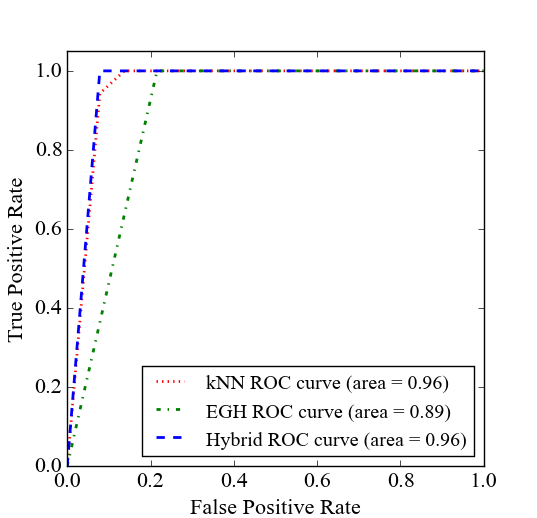
\includegraphics[width=0.5\textwidth]{adlfigs/study11ROC_02042014.png} &
		\tabularnewline
		((b)\tabularnewline
		\end{tabular}
		}
	\caption{
	ROC curve of house occupancy prediction in Study11 (02/04/2014).
}
	\label{fig_rocresults_2}
\end{figure}

\begin{figure}[h]
	\centering{
		\begin{tabular}{cccc}		
		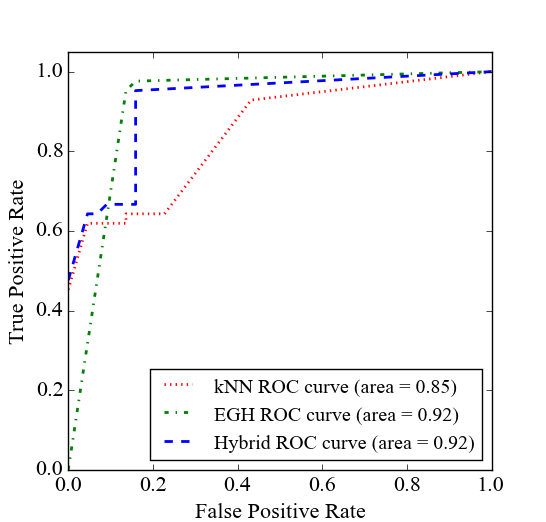
\includegraphics[width=0.5\textwidth]{adlfigs/study14ROC_12202013.png}
		\tabularnewline
		(c) \tabularnewline
		\end{tabular}
		}
	\caption{
	ROC curve of house occupancy prediction in (c) Study14 (12/20/2013).
}
	\label{fig_rocresults_3}
\end{figure}
\begin{figure}[h]
	\centering{
		\begin{tabular}{cccc}		
		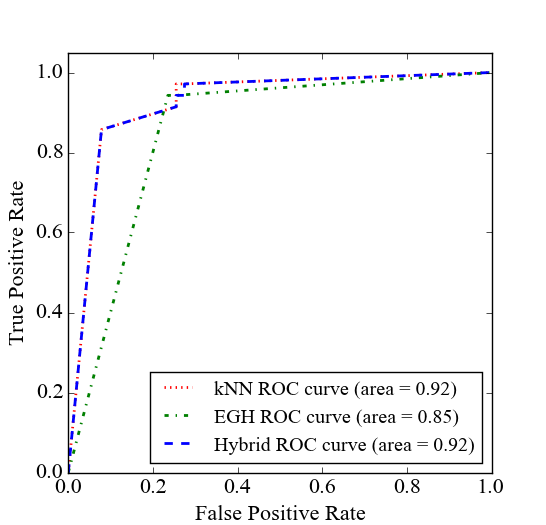
\includegraphics[width=0.6\textwidth]{adlfigs/study10ROC_02202014.png} &
		\tabularnewline
		(a)\tabularnewline
		\end{tabular}
		}
	\caption{
	ROC curve of house occupancy prediction in Study10 (02/20/2014).}
	\label{fig_rocresults_1}
\end{figure}

\begin{figure}[h]
	\centering{
		\begin{tabular}{cccc}		
		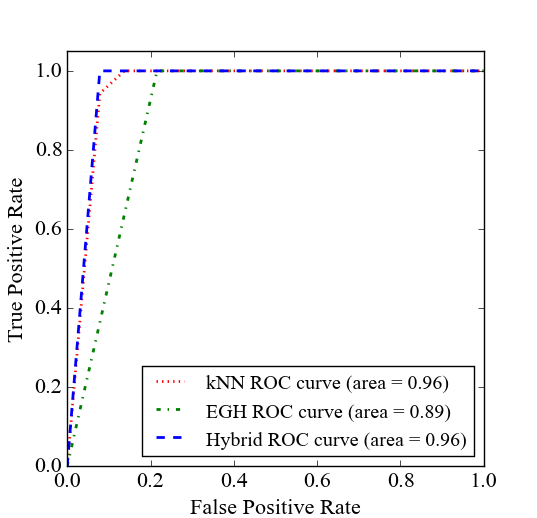
\includegraphics[width=0.6\textwidth]{adlfigs/study11ROC_02042014.png} &
		\tabularnewline
		((b)\tabularnewline
		\end{tabular}
		}
	\caption{
	ROC curve of house occupancy prediction in Study11 (02/04/2014).
}
	\label{fig_rocresults_2}
\end{figure}

\begin{figure}[h]
	\centering{
		\begin{tabular}{cccc}		
		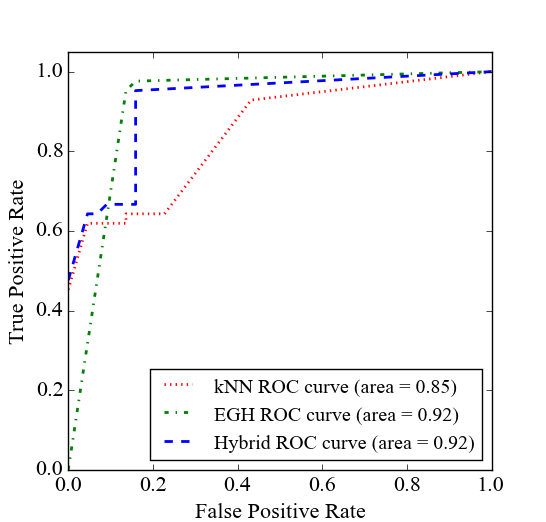
\includegraphics[width=0.6\textwidth]{adlfigs/study14ROC_12202013.png}
		\tabularnewline
		(c) \tabularnewline
		\end{tabular}
		}
	\caption{
	ROC curve of house occupancy prediction in (c) Study14 (12/20/2013).
}
	\label{fig_rocresults_3}
\end{figure}



%Also, we compare the 30 minutes whole house precision/recall/f-measure with the ROC curve, 
%the kNN ROC has a larger area even if EGH approach performs better on study10 and study11. 

%It depicts that ROC curve of mixture EGH model occupied larger area 0.92 than that from kNN approach 0.85. 
%We observe that although the precision/recall/fmeasure values are very close as in table~\ref{tab_individualResults}. 
%This hints that although the precision/recall/fmeasure results are competitive, 
%mixture EGH model can separate the occupancy and un-occupancy more sharply. 



%There are three test days in the dataset study14, 
%EGH outperforms kNN on the first day. 
%It's a tie on the second day. 
%The only exception on these datasets is the last day's experiment on study14, 
%kNN performs better because EGH mixture model currently
%only works on one-time even prediction. 



\section{Conclusion}
Due to urbanization, various aspects of people's lives, such as traffic flow, power consumption, air quality, and social network, change rapidly. In recent years, policy-makers and scientists have realized the urgent need for a transition to an environmentally friendly and sustainable city, and have proposed \emph{urban computing} research. One of the critical components of intelligent cities is smart building research. In particular, energy distribution and consumption are important topics because of their two-fold impact on society. First, power is an essential resource which has a great impact on our economy, so effective consumption is important. Secondly, the large impact the energy industry has on the environment, such as climate change, makes it an extremely sensitive and relevant topic of research. 

The central theme of this paper is using data analytics methods to tackle major issues in smart building. We provide a general framework and propose analytical solutions within that framework. The data mining techniques we use for discovering knowledge from the datasets are temporal mining and probabilistic models. We classify smart building events into two categories: device-related profiles and human-related events. This paper provides strategies to handle these two challenging energy-related problems. 

\begin{itemize}
\item \textbf{Characterization of electrical devices by energy disaggregation}: We studied energy consumption inside a building with an non-intrusive approach,  extracted the hidden patterns, and disclosed the correlation among these patterns. Furthermore, we connected these patterns with devices to infer the electricity usage of individual devices. 
We demonstrate that with the use of frequent-episode mining in conjunction with temporal mining techniques, we can effectively glean insights into usage patterns of electrical devices. Our approach describes a novel motif discovery approach that utilizes on/off events to unravel the operation frequency and duration of devices. We show that the our approach is very adroit at discerning multiple power levels and at effectively untwining the combinatorial operation of the devices. Moreover, we also show that this approach is not just an aid to disaggregation but, as a byproduct, also extracts temporal episodic relationships that shed insight into consumption patterns.

%\item \textbf{Characterization of water use ends by water disaggregation}: We characterized the water usage patterns inside a building, and inferred underlying water use ends. Additionally, we associated these patterns according to time to derive the activities of the people inside. 
%To improve upon our initial work, we propose a semi-supervised recursive multivariate piecewise motif mining approach for both energy and water disaggregation. Since the algorithm operates in two phases and effectively filters out appliances that have a large power consumption in the first stage, it can effectively discover usage patterns of smaller appliances. This insight provided by our approach allows for more precise energy disaggregation. Moreover, this approach can be effectively utilized to identify continuously variable loads, like outdoor heating. Similarly, by regarding hot and cold water as two phases, we can separate many water use ends.  

\item \textbf{Characterization of activities of daily life by occupancy prediction}: We investigated the activities patterns of people inside a residential building. Then we connected these patterns with a graphical model. Using the graphical model, we inferred whether the room/house was occupied. 
We demonstrate that by integrating the mixture EGH model and 
kNN together as a hybrid approach, we get the best prediction result. In our work, we formulate the problem as one of temporal mining; the activities inside the building are abstracted as episodes, and each episode is connected with an episode-generative HMM model. We mine the activity patterns according to the time and gap; both the duration of each type of activity, and the gap between two consecutive events are limited to be within a proper range. 
\end{itemize}

This research demonstrates that data analysis methods are able to solve smart building challenges. The proposed heuristic approaches utilize the characteristics of two typical profiles in smart buildings, thereby fundamentally paving the way to advanced controlling and scheduling systems for devices inside the buildings. 

%========
%In this day and age of big data and big compute, data mining is an important tool  the world. Technologies like Internet of Things and the availability of data such as traffic flow, power consumption, air quality, social networks, etc. have made \emph{urban computing} a burgeoning research topic. One of the critical components of \emph{urban computing} research is the analysis of smart buildings. Particularly, energy disaggregation and distribution are important topics because of its two-fold impact on society. Firstly it is an essential resource, which has a great impact on our economy so effective distribution is important. Secondly, the larger impact the energy industry has on the environment, like climate change, makes it an extremely sensitive and relevant topic of research. Thus, in this work, we focus on two important energy related problems in a smart building setting viz. resource disaggregation and occupancy prediction. 

\textbf{Future Work}

This paper has opened up many opportunities for future work. From a theoretical perspective, 
the probabilistic model of piecewise events has great research potential. We can try to connect frequent piecewise episodes with a generalized probabilistic model, as in \cite{laxman2005discovering}. %Furthermore, we can associate the dynamic time-warping models used in water disaggregation with similar probabilistic models. 

%In the aspect of research topics, the possible future works are stated as following. 
While we have made significant headway in energy disaggregation, there is significant room for improvement. One of the immediate extensions is to incorporate more features (in the multi-phase aggregate) when a device turns on. The sudden spikes in the aggregated data, when normalized, can indicate the \emph{startup shape}, which can be correlated to a device, and hence improve the overall effectiveness of device prediction, thus leading to more accurate energy disaggregation. Moreover, we can significantly improve the temporal mining approach to disaggregate more devices. Furthermore, our disaggregation algorithms can be explored for water disaggregation as well. We will exploit our temporal mining algorithms, integrated with dynamic time warping and motif mining, to propose an algorithm to effectively conduct home-level disaggregation. We can also extend our disaggregation algorithms for bandwidth distribution for internet service providers. Using our disaggregation algorithms, we can decipher the device-level internet usage and plan for effective distribution to a home/neighborhood. 

Solving energy disaggregation is an important practical problem, which, when resolved, results in a highly monetizable insight: consumption patterns. As a result, policy makers and energy distributors can design packages for consumers based on their needs. This will enable both consumers and distributors to effectively and \emph{smartly} buy and sell power that is highly customized to the needs of a home.


The occupancy prediction work lends itself to future extensions via hybrid approaches. We can integrate kNN and a mixture of EGH, which has the best performance on the sensor data set. One of the future directions is to incorporate GPS-based information to track movements of the house residents. This has the potential to be an excellent surrogate to automated power control of devices in a home. Another interesting problem to tackle is holiday occupancy prediction. The occupancy patterns for these days are completely different. For example, on certain weekdays, a person may never go out. Therefore the occupancy prediction probably depend more on date than on other indoor activities. 

One of the critical problems to ensure that we can reduce high energy consumption by automatically controlling the temperature regulation systems. Moreover, with the advent of more mainstream technologies like \emph{Nest} and other intelligent automatic control systems that remotely control the thermostat, occupancy prediction is a crucial parameter in determining the settings. Furthermore, comfort levels based on individuals can determine the temperature at which different parts of the residence should be set. Thus optimizing energy usage and maximizing user comfort are very important and immediate problems to solve.

Research in the domain of energy consumption has a two-fold impact on the society we live in. The rapid urbanization of our society requires the \emph{smart} and optimized distribution of power to meet the demands of the city. Logistical problems in power distribution, particularly meeting the high-volume requirement with minimal failure, are important problems. Moreover, the larger problem here is to ensure that we leave a small carbon foot print. Even though renewable energy resources are being tapped, fossil fuels are still the fundamental source of energy in our society. The optimized distribution of power and a well-established balance between supply and demand can ensure that we use only just as much of the fossil fuels as we need. As responsible researchers, it is important that we turn our talents towards this overarching goal of saving our planet and doing every thing we can to ensure that it is in good shape when we hand it over to our next generation.


\bibliographystyle{ACM-Reference-Format}
\bibliography{references} 

\end{document}
